%Chapter 4
\chapter{Results and validation}
\thispagestyle{empty}
\vspace{38em}
\hrulefill
\\
\enquote*{\textit{Quote.}} - Somebody\\
\newpage
\section{Introduction}
This section will discuss the results of the implementing the simulation methodology on various case case study. Further, the result of various simulated scenarios will be discussed. Finally validation of the the simulated scenarios using actual measurable tests will be discussed.
\section{Case study A \tiny{\color{blue}(Beatrix 123)}}

\subsection{System investigation}
Case study A represents a group of three gold mining shafts and a gold processing plant in the Free state that share a compressed air network. Prior to this study, efforts were made to optimise the system through \gls{dsm} energy projects. An investigation into the system was performed to identify potential energy and operation improvements strategies that are still available.
\par 
An air distribution layout was developed for the system, the simplified diagram is shown in Figure \ref{fig: Beatrix Air layout}.From this along with information from the mine personal and system data, an understanding of the operation philosophy was obtained. 
\par 
\begin{figure}[h!]
	\centering
	\fbox{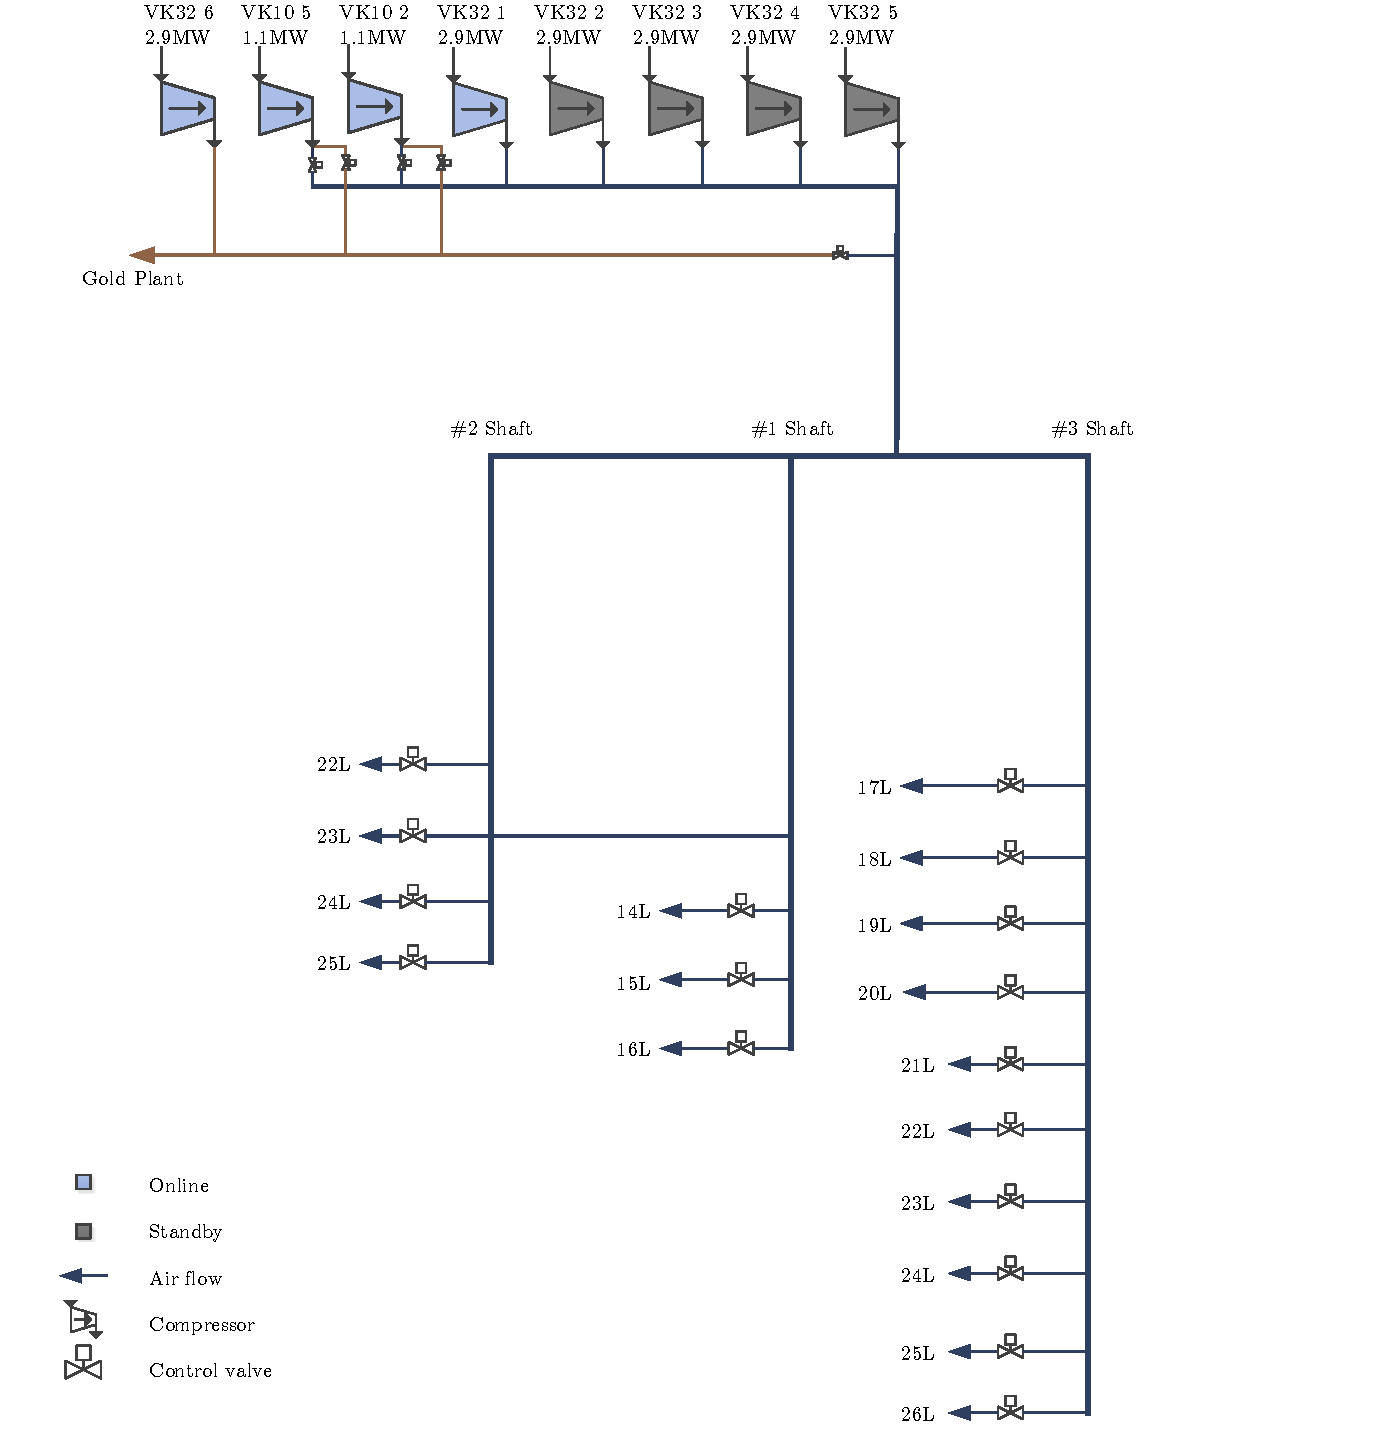
\includegraphics[trim =0cm 0.6cm 0cm 0.6cm,width=\textwidth]{Graphs/4/BeatLayout1/BeatLayout1.pdf}}
	\caption{Simplified process flow chart of the compressed air network.}
	\label{fig: Beatrix Air layout}
\end{figure}

The system typically uses 5 $MW$ of power, which increases by a 1 $MW$ during the drilling shift. The average weekday power profile is shown Figure \ref{fig: Beatrix power baseline}. Seven compresses are available in the system. Five large compressors (VK32s) rated at 2.9 $MW$ each and two smaller compressors (VK10) with a power rating of 1.1 $MW$ each. The system is normally operated with a combination of two VK32 compressors and two VK 10 compressors. The other compressors serve as standby. 
\begin{figure}[h!]
	\centering
	% GNUPLOT: LaTeX picture with Postscript
\begingroup
  \makeatletter
  \providecommand\color[2][]{%
    \GenericError{(gnuplot) \space\space\space\@spaces}{%
      Package color not loaded in conjunction with
      terminal option `colourtext'%
    }{See the gnuplot documentation for explanation.%
    }{Either use 'blacktext' in gnuplot or load the package
      color.sty in LaTeX.}%
    \renewcommand\color[2][]{}%
  }%
  \providecommand\includegraphics[2][]{%
    \GenericError{(gnuplot) \space\space\space\@spaces}{%
      Package graphicx or graphics not loaded%
    }{See the gnuplot documentation for explanation.%
    }{The gnuplot epslatex terminal needs graphicx.sty or graphics.sty.}%
    \renewcommand\includegraphics[2][]{}%
  }%
  \providecommand\rotatebox[2]{#2}%
  \@ifundefined{ifGPcolor}{%
    \newif\ifGPcolor
    \GPcolortrue
  }{}%
  \@ifundefined{ifGPblacktext}{%
    \newif\ifGPblacktext
    \GPblacktextfalse
  }{}%
  % define a \g@addto@macro without @ in the name:
  \let\gplgaddtomacro\g@addto@macro
  % define empty templates for all commands taking text:
  \gdef\gplbacktext{}%
  \gdef\gplfronttext{}%
  \makeatother
  \ifGPblacktext
    % no textcolor at all
    \def\colorrgb#1{}%
    \def\colorgray#1{}%
  \else
    % gray or color?
    \ifGPcolor
      \def\colorrgb#1{\color[rgb]{#1}}%
      \def\colorgray#1{\color[gray]{#1}}%
      \expandafter\def\csname LTw\endcsname{\color{white}}%
      \expandafter\def\csname LTb\endcsname{\color{black}}%
      \expandafter\def\csname LTa\endcsname{\color{black}}%
      \expandafter\def\csname LT0\endcsname{\color[rgb]{1,0,0}}%
      \expandafter\def\csname LT1\endcsname{\color[rgb]{0,1,0}}%
      \expandafter\def\csname LT2\endcsname{\color[rgb]{0,0,1}}%
      \expandafter\def\csname LT3\endcsname{\color[rgb]{1,0,1}}%
      \expandafter\def\csname LT4\endcsname{\color[rgb]{0,1,1}}%
      \expandafter\def\csname LT5\endcsname{\color[rgb]{1,1,0}}%
      \expandafter\def\csname LT6\endcsname{\color[rgb]{0,0,0}}%
      \expandafter\def\csname LT7\endcsname{\color[rgb]{1,0.3,0}}%
      \expandafter\def\csname LT8\endcsname{\color[rgb]{0.5,0.5,0.5}}%
    \else
      % gray
      \def\colorrgb#1{\color{black}}%
      \def\colorgray#1{\color[gray]{#1}}%
      \expandafter\def\csname LTw\endcsname{\color{white}}%
      \expandafter\def\csname LTb\endcsname{\color{black}}%
      \expandafter\def\csname LTa\endcsname{\color{black}}%
      \expandafter\def\csname LT0\endcsname{\color{black}}%
      \expandafter\def\csname LT1\endcsname{\color{black}}%
      \expandafter\def\csname LT2\endcsname{\color{black}}%
      \expandafter\def\csname LT3\endcsname{\color{black}}%
      \expandafter\def\csname LT4\endcsname{\color{black}}%
      \expandafter\def\csname LT5\endcsname{\color{black}}%
      \expandafter\def\csname LT6\endcsname{\color{black}}%
      \expandafter\def\csname LT7\endcsname{\color{black}}%
      \expandafter\def\csname LT8\endcsname{\color{black}}%
    \fi
  \fi
    \setlength{\unitlength}{0.0500bp}%
    \ifx\gptboxheight\undefined%
      \newlength{\gptboxheight}%
      \newlength{\gptboxwidth}%
      \newsavebox{\gptboxtext}%
    \fi%
    \setlength{\fboxrule}{0.5pt}%
    \setlength{\fboxsep}{1pt}%
\begin{picture}(9360.00,3024.00)%
    \gplgaddtomacro\gplbacktext{%
      \colorrgb{0.00,0.00,0.00}%
      \put(550,704){\makebox(0,0)[r]{\strut{}$0$}}%
      \colorrgb{0.00,0.00,0.00}%
      \put(550,1047){\makebox(0,0)[r]{\strut{}$1$}}%
      \colorrgb{0.00,0.00,0.00}%
      \put(550,1389){\makebox(0,0)[r]{\strut{}$2$}}%
      \colorrgb{0.00,0.00,0.00}%
      \put(550,1732){\makebox(0,0)[r]{\strut{}$3$}}%
      \colorrgb{0.00,0.00,0.00}%
      \put(550,2074){\makebox(0,0)[r]{\strut{}$4$}}%
      \colorrgb{0.00,0.00,0.00}%
      \put(550,2417){\makebox(0,0)[r]{\strut{}$5$}}%
      \colorrgb{0.00,0.00,0.00}%
      \put(550,2759){\makebox(0,0)[r]{\strut{}$6$}}%
      \colorrgb{0.00,0.00,0.00}%
      \put(682,484){\makebox(0,0){\strut{}00:00}}%
      \colorrgb{0.00,0.00,0.00}%
      \put(2062,484){\makebox(0,0){\strut{}04:00}}%
      \colorrgb{0.00,0.00,0.00}%
      \put(3442,484){\makebox(0,0){\strut{}08:00}}%
      \colorrgb{0.00,0.00,0.00}%
      \put(4822,484){\makebox(0,0){\strut{}12:00}}%
      \colorrgb{0.00,0.00,0.00}%
      \put(6202,484){\makebox(0,0){\strut{}16:00}}%
      \colorrgb{0.00,0.00,0.00}%
      \put(7582,484){\makebox(0,0){\strut{}20:00}}%
      \colorrgb{0.00,0.00,0.00}%
      \put(8962,484){\makebox(0,0){\strut{}00:00}}%
    }%
    \gplgaddtomacro\gplfronttext{%
      \csname LTb\endcsname%
      \put(176,1731){\rotatebox{-270}{\makebox(0,0){\strut{}Power $(MW)$}}}%
      \put(4822,154){\makebox(0,0){\strut{}Time of Day}}%
    }%
    \gplbacktext
    \put(0,0){\fbox{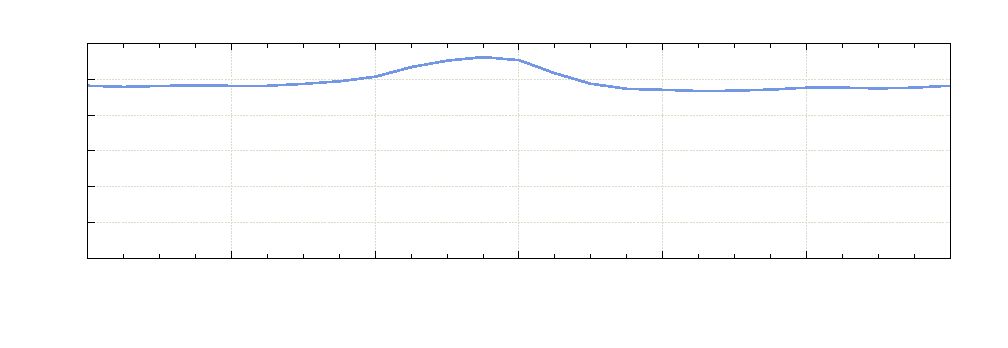
\includegraphics[trim=0 0 0.1cm 0, clip]{Graphs/4/BeetBaseline/Power/Power}}}%
    \gplfronttext
  \end{picture}%
\endgroup

	\caption{Average power profile}
	\label{fig: Beatrix power baseline}
\end{figure}

\par
Air is supplied to the sections in three mining shafts as well as a gold processing plant on the surface.  The mine normally operates the compressors with a constant pressure set-point f 500 \gls{kpa}.  The set-point is  kept this high as the gold processing plant requires constant high pressure throughout the day. This makes it difficult to reduce the set-points of the compressor.
\par
 It is possible to control the air supply pressure to the gold plant independently from the rest of the network. This is performed by utilising the surface control valves and a specific configuration of compressors. The mine prefers not to operate this way.
\subsection{Model development}
With the data and understanding of the gathered from the investigation, a model was developed in the \gls{ptb} tool using the methodology discussed in Chapter 3. First the simulation boundary was selected to include the measured flows to each level as well as the processing plant. As data was only available in half an hour intervals, the simulation step size was was set to 30 minutes to match the available data.
\par
Component models were developed using the respective methods discussed in chapter 3. The following assumption were  made to simplify the development the model:
\begin{itemize}
	\item The effect of compressor after cooling was negligible
	\item Heat transfer over the pipe length was negligible
	\item Underground temperature and humidity remained constant for each level
	\item Surface ambient air conditions followed the average summer trend
\end{itemize} 
The model components was calibrated so that the simulated outputs matched data from the real system.
\subsubsection{Verification of model}
Verification was performed to ensure that simulated output accuracy was >95\%. Figure \ref{fig: Verification Power Beatrix} and Figure \ref{fig: Verification Flow Beatrix} compare the to total simulated and actual power and flow respectively. The average accuracy was 97.34\% for system power and  97.01\% for system flow. Both these parameters were well within the target 95\% accuracy.
\begin{figure}[h]
	\centering
	% GNUPLOT: LaTeX picture with Postscript
\begingroup
  \makeatletter
  \providecommand\color[2][]{%
    \GenericError{(gnuplot) \space\space\space\@spaces}{%
      Package color not loaded in conjunction with
      terminal option `colourtext'%
    }{See the gnuplot documentation for explanation.%
    }{Either use 'blacktext' in gnuplot or load the package
      color.sty in LaTeX.}%
    \renewcommand\color[2][]{}%
  }%
  \providecommand\includegraphics[2][]{%
    \GenericError{(gnuplot) \space\space\space\@spaces}{%
      Package graphicx or graphics not loaded%
    }{See the gnuplot documentation for explanation.%
    }{The gnuplot epslatex terminal needs graphicx.sty or graphics.sty.}%
    \renewcommand\includegraphics[2][]{}%
  }%
  \providecommand\rotatebox[2]{#2}%
  \@ifundefined{ifGPcolor}{%
    \newif\ifGPcolor
    \GPcolortrue
  }{}%
  \@ifundefined{ifGPblacktext}{%
    \newif\ifGPblacktext
    \GPblacktextfalse
  }{}%
  % define a \g@addto@macro without @ in the name:
  \let\gplgaddtomacro\g@addto@macro
  % define empty templates for all commands taking text:
  \gdef\gplbacktext{}%
  \gdef\gplfronttext{}%
  \makeatother
  \ifGPblacktext
    % no textcolor at all
    \def\colorrgb#1{}%
    \def\colorgray#1{}%
  \else
    % gray or color?
    \ifGPcolor
      \def\colorrgb#1{\color[rgb]{#1}}%
      \def\colorgray#1{\color[gray]{#1}}%
      \expandafter\def\csname LTw\endcsname{\color{white}}%
      \expandafter\def\csname LTb\endcsname{\color{black}}%
      \expandafter\def\csname LTa\endcsname{\color{black}}%
      \expandafter\def\csname LT0\endcsname{\color[rgb]{1,0,0}}%
      \expandafter\def\csname LT1\endcsname{\color[rgb]{0,1,0}}%
      \expandafter\def\csname LT2\endcsname{\color[rgb]{0,0,1}}%
      \expandafter\def\csname LT3\endcsname{\color[rgb]{1,0,1}}%
      \expandafter\def\csname LT4\endcsname{\color[rgb]{0,1,1}}%
      \expandafter\def\csname LT5\endcsname{\color[rgb]{1,1,0}}%
      \expandafter\def\csname LT6\endcsname{\color[rgb]{0,0,0}}%
      \expandafter\def\csname LT7\endcsname{\color[rgb]{1,0.3,0}}%
      \expandafter\def\csname LT8\endcsname{\color[rgb]{0.5,0.5,0.5}}%
    \else
      % gray
      \def\colorrgb#1{\color{black}}%
      \def\colorgray#1{\color[gray]{#1}}%
      \expandafter\def\csname LTw\endcsname{\color{white}}%
      \expandafter\def\csname LTb\endcsname{\color{black}}%
      \expandafter\def\csname LTa\endcsname{\color{black}}%
      \expandafter\def\csname LT0\endcsname{\color{black}}%
      \expandafter\def\csname LT1\endcsname{\color{black}}%
      \expandafter\def\csname LT2\endcsname{\color{black}}%
      \expandafter\def\csname LT3\endcsname{\color{black}}%
      \expandafter\def\csname LT4\endcsname{\color{black}}%
      \expandafter\def\csname LT5\endcsname{\color{black}}%
      \expandafter\def\csname LT6\endcsname{\color{black}}%
      \expandafter\def\csname LT7\endcsname{\color{black}}%
      \expandafter\def\csname LT8\endcsname{\color{black}}%
    \fi
  \fi
    \setlength{\unitlength}{0.0500bp}%
    \ifx\gptboxheight\undefined%
      \newlength{\gptboxheight}%
      \newlength{\gptboxwidth}%
      \newsavebox{\gptboxtext}%
    \fi%
    \setlength{\fboxrule}{0.5pt}%
    \setlength{\fboxsep}{1pt}%
\begin{picture}(9360.00,4032.00)%
    \gplgaddtomacro\gplbacktext{%
      \colorrgb{0.00,0.00,0.00}%
      \put(550,924){\makebox(0,0)[r]{\strut{}$0$}}%
      \colorrgb{0.00,0.00,0.00}%
      \put(550,1279){\makebox(0,0)[r]{\strut{}$1$}}%
      \colorrgb{0.00,0.00,0.00}%
      \put(550,1635){\makebox(0,0)[r]{\strut{}$2$}}%
      \colorrgb{0.00,0.00,0.00}%
      \put(550,1990){\makebox(0,0)[r]{\strut{}$3$}}%
      \colorrgb{0.00,0.00,0.00}%
      \put(550,2346){\makebox(0,0)[r]{\strut{}$4$}}%
      \colorrgb{0.00,0.00,0.00}%
      \put(550,2701){\makebox(0,0)[r]{\strut{}$5$}}%
      \colorrgb{0.00,0.00,0.00}%
      \put(550,3056){\makebox(0,0)[r]{\strut{}$6$}}%
      \colorrgb{0.00,0.00,0.00}%
      \put(550,3412){\makebox(0,0)[r]{\strut{}$7$}}%
      \colorrgb{0.00,0.00,0.00}%
      \put(550,3767){\makebox(0,0)[r]{\strut{}$8$}}%
      \colorrgb{0.00,0.00,0.00}%
      \put(682,704){\makebox(0,0){\strut{}00:00}}%
      \colorrgb{0.00,0.00,0.00}%
      \put(1937,704){\makebox(0,0){\strut{}04:00}}%
      \colorrgb{0.00,0.00,0.00}%
      \put(3193,704){\makebox(0,0){\strut{}08:00}}%
      \colorrgb{0.00,0.00,0.00}%
      \put(4448,704){\makebox(0,0){\strut{}12:00}}%
      \colorrgb{0.00,0.00,0.00}%
      \put(5703,704){\makebox(0,0){\strut{}16:00}}%
      \colorrgb{0.00,0.00,0.00}%
      \put(6959,704){\makebox(0,0){\strut{}20:00}}%
      \colorrgb{0.00,0.00,0.00}%
      \put(8214,704){\makebox(0,0){\strut{}00:00}}%
      \colorrgb{0.00,0.00,0.00}%
      \put(8346,924){\makebox(0,0)[l]{\strut{}$0$}}%
      \colorrgb{0.00,0.00,0.00}%
      \put(8346,2061){\makebox(0,0)[l]{\strut{}$10$}}%
      \colorrgb{0.00,0.00,0.00}%
      \put(8346,3198){\makebox(0,0)[l]{\strut{}$20$}}%
    }%
    \gplgaddtomacro\gplfronttext{%
      \csname LTb\endcsname%
      \put(176,2345){\rotatebox{-270}{\makebox(0,0){\strut{}Power $(MW)$}}}%
      \put(8851,2345){\rotatebox{-270}{\makebox(0,0){\strut{}$\%$ $error$}}}%
      \put(4448,374){\makebox(0,0){\strut{}Time of use}}%
      \csname LTb\endcsname%
      \put(2175,173){\makebox(0,0)[r]{\strut{}Baseline power}}%
      \csname LTb\endcsname%
      \put(5010,173){\makebox(0,0)[r]{\strut{}Simulated power}}%
      \csname LTb\endcsname%
      \put(7700,173){\makebox(0,0)[r]{\strut{}Rel. Error}}%
    }%
    \gplbacktext
    \put(0,0){\fbox{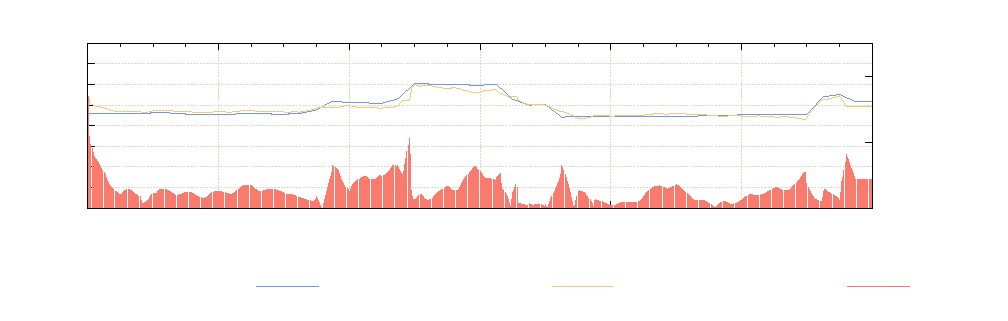
\includegraphics[trim=0 0 0.1cm 0, clip]{Graphs/4/BeetVerify/Power/Power}}}%
    \gplfronttext
  \end{picture}%
\endgroup

	\caption{The simulated power compared to the actual measured power}
	\label{fig: Verification Power Beatrix}
\end{figure}

\begin{figure}[h]
	\centering
	% GNUPLOT: LaTeX picture with Postscript
\begingroup
  \makeatletter
  \providecommand\color[2][]{%
    \GenericError{(gnuplot) \space\space\space\@spaces}{%
      Package color not loaded in conjunction with
      terminal option `colourtext'%
    }{See the gnuplot documentation for explanation.%
    }{Either use 'blacktext' in gnuplot or load the package
      color.sty in LaTeX.}%
    \renewcommand\color[2][]{}%
  }%
  \providecommand\includegraphics[2][]{%
    \GenericError{(gnuplot) \space\space\space\@spaces}{%
      Package graphicx or graphics not loaded%
    }{See the gnuplot documentation for explanation.%
    }{The gnuplot epslatex terminal needs graphicx.sty or graphics.sty.}%
    \renewcommand\includegraphics[2][]{}%
  }%
  \providecommand\rotatebox[2]{#2}%
  \@ifundefined{ifGPcolor}{%
    \newif\ifGPcolor
    \GPcolortrue
  }{}%
  \@ifundefined{ifGPblacktext}{%
    \newif\ifGPblacktext
    \GPblacktextfalse
  }{}%
  % define a \g@addto@macro without @ in the name:
  \let\gplgaddtomacro\g@addto@macro
  % define empty templates for all commands taking text:
  \gdef\gplbacktext{}%
  \gdef\gplfronttext{}%
  \makeatother
  \ifGPblacktext
    % no textcolor at all
    \def\colorrgb#1{}%
    \def\colorgray#1{}%
  \else
    % gray or color?
    \ifGPcolor
      \def\colorrgb#1{\color[rgb]{#1}}%
      \def\colorgray#1{\color[gray]{#1}}%
      \expandafter\def\csname LTw\endcsname{\color{white}}%
      \expandafter\def\csname LTb\endcsname{\color{black}}%
      \expandafter\def\csname LTa\endcsname{\color{black}}%
      \expandafter\def\csname LT0\endcsname{\color[rgb]{1,0,0}}%
      \expandafter\def\csname LT1\endcsname{\color[rgb]{0,1,0}}%
      \expandafter\def\csname LT2\endcsname{\color[rgb]{0,0,1}}%
      \expandafter\def\csname LT3\endcsname{\color[rgb]{1,0,1}}%
      \expandafter\def\csname LT4\endcsname{\color[rgb]{0,1,1}}%
      \expandafter\def\csname LT5\endcsname{\color[rgb]{1,1,0}}%
      \expandafter\def\csname LT6\endcsname{\color[rgb]{0,0,0}}%
      \expandafter\def\csname LT7\endcsname{\color[rgb]{1,0.3,0}}%
      \expandafter\def\csname LT8\endcsname{\color[rgb]{0.5,0.5,0.5}}%
    \else
      % gray
      \def\colorrgb#1{\color{black}}%
      \def\colorgray#1{\color[gray]{#1}}%
      \expandafter\def\csname LTw\endcsname{\color{white}}%
      \expandafter\def\csname LTb\endcsname{\color{black}}%
      \expandafter\def\csname LTa\endcsname{\color{black}}%
      \expandafter\def\csname LT0\endcsname{\color{black}}%
      \expandafter\def\csname LT1\endcsname{\color{black}}%
      \expandafter\def\csname LT2\endcsname{\color{black}}%
      \expandafter\def\csname LT3\endcsname{\color{black}}%
      \expandafter\def\csname LT4\endcsname{\color{black}}%
      \expandafter\def\csname LT5\endcsname{\color{black}}%
      \expandafter\def\csname LT6\endcsname{\color{black}}%
      \expandafter\def\csname LT7\endcsname{\color{black}}%
      \expandafter\def\csname LT8\endcsname{\color{black}}%
    \fi
  \fi
    \setlength{\unitlength}{0.0500bp}%
    \ifx\gptboxheight\undefined%
      \newlength{\gptboxheight}%
      \newlength{\gptboxwidth}%
      \newsavebox{\gptboxtext}%
    \fi%
    \setlength{\fboxrule}{0.5pt}%
    \setlength{\fboxsep}{1pt}%
\begin{picture}(9360.00,4032.00)%
    \gplgaddtomacro\gplbacktext{%
      \colorrgb{0.00,0.00,0.00}%
      \put(682,924){\makebox(0,0)[r]{\strut{}$0$}}%
      \colorrgb{0.00,0.00,0.00}%
      \put(682,1872){\makebox(0,0)[r]{\strut{}$5$}}%
      \colorrgb{0.00,0.00,0.00}%
      \put(682,2819){\makebox(0,0)[r]{\strut{}$10$}}%
      \colorrgb{0.00,0.00,0.00}%
      \put(682,3767){\makebox(0,0)[r]{\strut{}$15$}}%
      \colorrgb{0.00,0.00,0.00}%
      \put(814,704){\makebox(0,0){\strut{}00:00}}%
      \colorrgb{0.00,0.00,0.00}%
      \put(2047,704){\makebox(0,0){\strut{}04:00}}%
      \colorrgb{0.00,0.00,0.00}%
      \put(3281,704){\makebox(0,0){\strut{}08:00}}%
      \colorrgb{0.00,0.00,0.00}%
      \put(4514,704){\makebox(0,0){\strut{}12:00}}%
      \colorrgb{0.00,0.00,0.00}%
      \put(5747,704){\makebox(0,0){\strut{}16:00}}%
      \colorrgb{0.00,0.00,0.00}%
      \put(6981,704){\makebox(0,0){\strut{}20:00}}%
      \colorrgb{0.00,0.00,0.00}%
      \put(8214,704){\makebox(0,0){\strut{}00:00}}%
      \colorrgb{0.00,0.00,0.00}%
      \put(8346,924){\makebox(0,0)[l]{\strut{}$0$}}%
      \colorrgb{0.00,0.00,0.00}%
      \put(8346,2061){\makebox(0,0)[l]{\strut{}$10$}}%
      \colorrgb{0.00,0.00,0.00}%
      \put(8346,3198){\makebox(0,0)[l]{\strut{}$20$}}%
    }%
    \gplgaddtomacro\gplfronttext{%
      \csname LTb\endcsname%
      \put(176,2345){\rotatebox{-270}{\makebox(0,0){\strut{}Flow $(kg/s)$}}}%
      \put(8851,2345){\rotatebox{-270}{\makebox(0,0){\strut{}$\% error$}}}%
      \put(4514,374){\makebox(0,0){\strut{}Time of Day}}%
      \csname LTb\endcsname%
      \put(2307,173){\makebox(0,0)[r]{\strut{}Baseline flow}}%
      \csname LTb\endcsname%
      \put(5010,173){\makebox(0,0)[r]{\strut{}Simulated flow}}%
      \csname LTb\endcsname%
      \put(7713,173){\makebox(0,0)[r]{\strut{}Error}}%
    }%
    \gplbacktext
    \put(0,0){\fbox{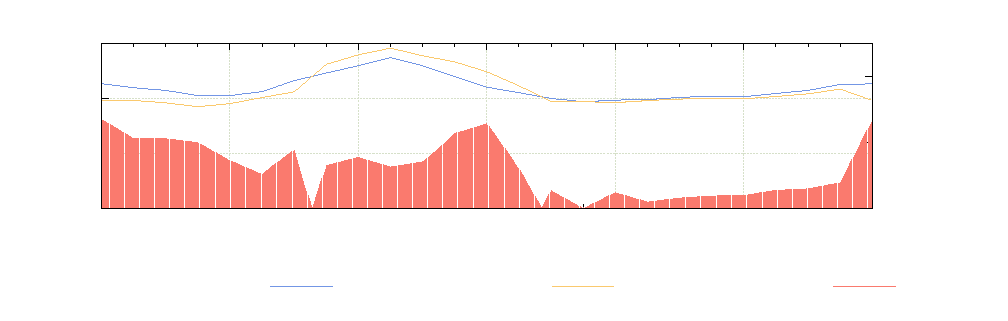
\includegraphics[trim=0 0 0.1cm 0, clip]{Graphs/4/BeetVerify/Flow/Flow}}}%
    \gplfronttext
  \end{picture}%
\endgroup

	\caption{The simulated flow compared to the actual measured flow}
	\label{fig: Verification Flow Beatrix}
\end{figure}
The same check was performed for the compressor outlet pressure. Figure \ref{fig: Verification Pressure Beatrix} compares the actual measured and simulated pressures. The accuracy of the outlet pressure was 99.1\%. The high accuracy of the simulated pressure was expected as the mine uses a constant pressure set-point for the compressors.
\begin{figure}[h]
	\centering
	% GNUPLOT: LaTeX picture with Postscript
\begingroup
  \makeatletter
  \providecommand\color[2][]{%
    \GenericError{(gnuplot) \space\space\space\@spaces}{%
      Package color not loaded in conjunction with
      terminal option `colourtext'%
    }{See the gnuplot documentation for explanation.%
    }{Either use 'blacktext' in gnuplot or load the package
      color.sty in LaTeX.}%
    \renewcommand\color[2][]{}%
  }%
  \providecommand\includegraphics[2][]{%
    \GenericError{(gnuplot) \space\space\space\@spaces}{%
      Package graphicx or graphics not loaded%
    }{See the gnuplot documentation for explanation.%
    }{The gnuplot epslatex terminal needs graphicx.sty or graphics.sty.}%
    \renewcommand\includegraphics[2][]{}%
  }%
  \providecommand\rotatebox[2]{#2}%
  \@ifundefined{ifGPcolor}{%
    \newif\ifGPcolor
    \GPcolortrue
  }{}%
  \@ifundefined{ifGPblacktext}{%
    \newif\ifGPblacktext
    \GPblacktextfalse
  }{}%
  % define a \g@addto@macro without @ in the name:
  \let\gplgaddtomacro\g@addto@macro
  % define empty templates for all commands taking text:
  \gdef\gplbacktext{}%
  \gdef\gplfronttext{}%
  \makeatother
  \ifGPblacktext
    % no textcolor at all
    \def\colorrgb#1{}%
    \def\colorgray#1{}%
  \else
    % gray or color?
    \ifGPcolor
      \def\colorrgb#1{\color[rgb]{#1}}%
      \def\colorgray#1{\color[gray]{#1}}%
      \expandafter\def\csname LTw\endcsname{\color{white}}%
      \expandafter\def\csname LTb\endcsname{\color{black}}%
      \expandafter\def\csname LTa\endcsname{\color{black}}%
      \expandafter\def\csname LT0\endcsname{\color[rgb]{1,0,0}}%
      \expandafter\def\csname LT1\endcsname{\color[rgb]{0,1,0}}%
      \expandafter\def\csname LT2\endcsname{\color[rgb]{0,0,1}}%
      \expandafter\def\csname LT3\endcsname{\color[rgb]{1,0,1}}%
      \expandafter\def\csname LT4\endcsname{\color[rgb]{0,1,1}}%
      \expandafter\def\csname LT5\endcsname{\color[rgb]{1,1,0}}%
      \expandafter\def\csname LT6\endcsname{\color[rgb]{0,0,0}}%
      \expandafter\def\csname LT7\endcsname{\color[rgb]{1,0.3,0}}%
      \expandafter\def\csname LT8\endcsname{\color[rgb]{0.5,0.5,0.5}}%
    \else
      % gray
      \def\colorrgb#1{\color{black}}%
      \def\colorgray#1{\color[gray]{#1}}%
      \expandafter\def\csname LTw\endcsname{\color{white}}%
      \expandafter\def\csname LTb\endcsname{\color{black}}%
      \expandafter\def\csname LTa\endcsname{\color{black}}%
      \expandafter\def\csname LT0\endcsname{\color{black}}%
      \expandafter\def\csname LT1\endcsname{\color{black}}%
      \expandafter\def\csname LT2\endcsname{\color{black}}%
      \expandafter\def\csname LT3\endcsname{\color{black}}%
      \expandafter\def\csname LT4\endcsname{\color{black}}%
      \expandafter\def\csname LT5\endcsname{\color{black}}%
      \expandafter\def\csname LT6\endcsname{\color{black}}%
      \expandafter\def\csname LT7\endcsname{\color{black}}%
      \expandafter\def\csname LT8\endcsname{\color{black}}%
    \fi
  \fi
    \setlength{\unitlength}{0.0500bp}%
    \ifx\gptboxheight\undefined%
      \newlength{\gptboxheight}%
      \newlength{\gptboxwidth}%
      \newsavebox{\gptboxtext}%
    \fi%
    \setlength{\fboxrule}{0.5pt}%
    \setlength{\fboxsep}{1pt}%
\begin{picture}(9360.00,2772.00)%
    \gplgaddtomacro\gplbacktext{%
      \colorrgb{0.00,0.00,0.00}%
      \put(814,924){\makebox(0,0)[r]{\strut{}$300$}}%
      \colorrgb{0.00,0.00,0.00}%
      \put(814,1452){\makebox(0,0)[r]{\strut{}$350$}}%
      \colorrgb{0.00,0.00,0.00}%
      \put(814,1979){\makebox(0,0)[r]{\strut{}$400$}}%
      \colorrgb{0.00,0.00,0.00}%
      \put(814,2507){\makebox(0,0)[r]{\strut{}$450$}}%
      \colorrgb{0.00,0.00,0.00}%
      \put(946,704){\makebox(0,0){\strut{}00:00}}%
      \colorrgb{0.00,0.00,0.00}%
      \put(2157,704){\makebox(0,0){\strut{}04:00}}%
      \colorrgb{0.00,0.00,0.00}%
      \put(3369,704){\makebox(0,0){\strut{}08:00}}%
      \colorrgb{0.00,0.00,0.00}%
      \put(4580,704){\makebox(0,0){\strut{}12:00}}%
      \colorrgb{0.00,0.00,0.00}%
      \put(5791,704){\makebox(0,0){\strut{}16:00}}%
      \colorrgb{0.00,0.00,0.00}%
      \put(7003,704){\makebox(0,0){\strut{}20:00}}%
      \colorrgb{0.00,0.00,0.00}%
      \put(8214,704){\makebox(0,0){\strut{}00:00}}%
      \colorrgb{0.00,0.00,0.00}%
      \put(8346,924){\makebox(0,0)[l]{\strut{}$0$}}%
      \colorrgb{0.00,0.00,0.00}%
      \put(8346,1557){\makebox(0,0)[l]{\strut{}$10$}}%
      \colorrgb{0.00,0.00,0.00}%
      \put(8346,2190){\makebox(0,0)[l]{\strut{}$20$}}%
    }%
    \gplgaddtomacro\gplfronttext{%
      \csname LTb\endcsname%
      \put(176,1715){\rotatebox{-270}{\makebox(0,0){\strut{}Pressure $(kPa)$}}}%
      \put(8851,1715){\rotatebox{-270}{\makebox(0,0){\strut{}$\% error$}}}%
      \put(4580,374){\makebox(0,0){\strut{}Time of Day}}%
      \csname LTb\endcsname%
      \put(2241,173){\makebox(0,0)[r]{\strut{}Baseline press.}}%
      \csname LTb\endcsname%
      \put(5208,173){\makebox(0,0)[r]{\strut{}Simulated press.}}%
      \csname LTb\endcsname%
      \put(8175,173){\makebox(0,0)[r]{\strut{}Error}}%
    }%
    \gplbacktext
    \put(0,0){
\includegraphics{Graphs/4/BeetVerify/Pressure/Pressure}}%
    \gplfronttext
  \end{picture}%
\endgroup

	\caption{The simulated Pressure compared to the actual measured pressure}
	\label{fig: Verification Pressure Beatrix}
\end{figure}
\par
The accuracy of the model was checked in more detail to ensure that each modelled parameter matched the actual measurement with high accuracy. Table \ref{Table: A verification} shows the accuracy each measured simulation output in the model. 
\subsection{Scenario 1. Compressor set points}
\begin{figure}[h!]
	\centering
	% GNUPLOT: LaTeX picture with Postscript
\begingroup
  \makeatletter
  \providecommand\color[2][]{%
    \GenericError{(gnuplot) \space\space\space\@spaces}{%
      Package color not loaded in conjunction with
      terminal option `colourtext'%
    }{See the gnuplot documentation for explanation.%
    }{Either use 'blacktext' in gnuplot or load the package
      color.sty in LaTeX.}%
    \renewcommand\color[2][]{}%
  }%
  \providecommand\includegraphics[2][]{%
    \GenericError{(gnuplot) \space\space\space\@spaces}{%
      Package graphicx or graphics not loaded%
    }{See the gnuplot documentation for explanation.%
    }{The gnuplot epslatex terminal needs graphicx.sty or graphics.sty.}%
    \renewcommand\includegraphics[2][]{}%
  }%
  \providecommand\rotatebox[2]{#2}%
  \@ifundefined{ifGPcolor}{%
    \newif\ifGPcolor
    \GPcolortrue
  }{}%
  \@ifundefined{ifGPblacktext}{%
    \newif\ifGPblacktext
    \GPblacktextfalse
  }{}%
  % define a \g@addto@macro without @ in the name:
  \let\gplgaddtomacro\g@addto@macro
  % define empty templates for all commands taking text:
  \gdef\gplbacktext{}%
  \gdef\gplfronttext{}%
  \makeatother
  \ifGPblacktext
    % no textcolor at all
    \def\colorrgb#1{}%
    \def\colorgray#1{}%
  \else
    % gray or color?
    \ifGPcolor
      \def\colorrgb#1{\color[rgb]{#1}}%
      \def\colorgray#1{\color[gray]{#1}}%
      \expandafter\def\csname LTw\endcsname{\color{white}}%
      \expandafter\def\csname LTb\endcsname{\color{black}}%
      \expandafter\def\csname LTa\endcsname{\color{black}}%
      \expandafter\def\csname LT0\endcsname{\color[rgb]{1,0,0}}%
      \expandafter\def\csname LT1\endcsname{\color[rgb]{0,1,0}}%
      \expandafter\def\csname LT2\endcsname{\color[rgb]{0,0,1}}%
      \expandafter\def\csname LT3\endcsname{\color[rgb]{1,0,1}}%
      \expandafter\def\csname LT4\endcsname{\color[rgb]{0,1,1}}%
      \expandafter\def\csname LT5\endcsname{\color[rgb]{1,1,0}}%
      \expandafter\def\csname LT6\endcsname{\color[rgb]{0,0,0}}%
      \expandafter\def\csname LT7\endcsname{\color[rgb]{1,0.3,0}}%
      \expandafter\def\csname LT8\endcsname{\color[rgb]{0.5,0.5,0.5}}%
    \else
      % gray
      \def\colorrgb#1{\color{black}}%
      \def\colorgray#1{\color[gray]{#1}}%
      \expandafter\def\csname LTw\endcsname{\color{white}}%
      \expandafter\def\csname LTb\endcsname{\color{black}}%
      \expandafter\def\csname LTa\endcsname{\color{black}}%
      \expandafter\def\csname LT0\endcsname{\color{black}}%
      \expandafter\def\csname LT1\endcsname{\color{black}}%
      \expandafter\def\csname LT2\endcsname{\color{black}}%
      \expandafter\def\csname LT3\endcsname{\color{black}}%
      \expandafter\def\csname LT4\endcsname{\color{black}}%
      \expandafter\def\csname LT5\endcsname{\color{black}}%
      \expandafter\def\csname LT6\endcsname{\color{black}}%
      \expandafter\def\csname LT7\endcsname{\color{black}}%
      \expandafter\def\csname LT8\endcsname{\color{black}}%
    \fi
  \fi
    \setlength{\unitlength}{0.0500bp}%
    \ifx\gptboxheight\undefined%
      \newlength{\gptboxheight}%
      \newlength{\gptboxwidth}%
      \newsavebox{\gptboxtext}%
    \fi%
    \setlength{\fboxrule}{0.5pt}%
    \setlength{\fboxsep}{1pt}%
\begin{picture}(9360.00,3780.00)%
    \gplgaddtomacro\gplbacktext{%
      \colorrgb{0.00,0.00,0.00}%
      \put(550,924){\makebox(0,0)[r]{\strut{}$0$}}%
      \colorrgb{0.00,0.00,0.00}%
      \put(550,1788){\makebox(0,0)[r]{\strut{}$2$}}%
      \colorrgb{0.00,0.00,0.00}%
      \put(550,2651){\makebox(0,0)[r]{\strut{}$4$}}%
      \colorrgb{0.00,0.00,0.00}%
      \put(550,3515){\makebox(0,0)[r]{\strut{}$6$}}%
      \colorrgb{0.00,0.00,0.00}%
      \put(682,704){\makebox(0,0){\strut{}00:00}}%
      \colorrgb{0.00,0.00,0.00}%
      \put(2062,704){\makebox(0,0){\strut{}04:00}}%
      \colorrgb{0.00,0.00,0.00}%
      \put(3442,704){\makebox(0,0){\strut{}08:00}}%
      \colorrgb{0.00,0.00,0.00}%
      \put(4822,704){\makebox(0,0){\strut{}12:00}}%
      \colorrgb{0.00,0.00,0.00}%
      \put(6202,704){\makebox(0,0){\strut{}16:00}}%
      \colorrgb{0.00,0.00,0.00}%
      \put(7582,704){\makebox(0,0){\strut{}20:00}}%
      \colorrgb{0.00,0.00,0.00}%
      \put(8962,704){\makebox(0,0){\strut{}00:00}}%
    }%
    \gplgaddtomacro\gplfronttext{%
      \csname LTb\endcsname%
      \put(176,2219){\rotatebox{-270}{\makebox(0,0){\strut{}Power $(MW)$}}}%
      \put(4822,374){\makebox(0,0){\strut{}Time of Day}}%
      \csname LTb\endcsname%
      \put(2747,173){\makebox(0,0)[r]{\strut{}Baseline}}%
      \csname LTb\endcsname%
      \put(5186,173){\makebox(0,0)[r]{\strut{}Intervention}}%
      \csname LTb\endcsname%
      \put(7625,173){\makebox(0,0)[r]{\strut{}Power saving}}%
    }%
    \gplbacktext
    \put(0,0){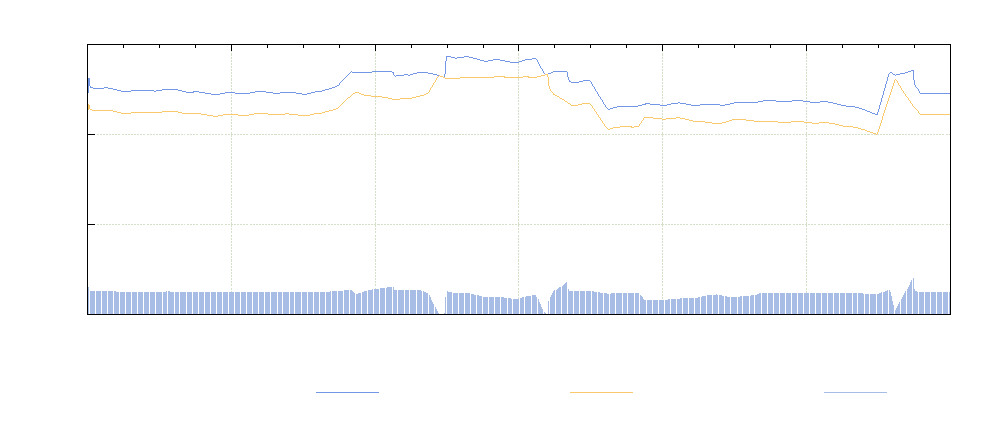
\includegraphics{Graphs/4/BeetResults/CompSetpoints/CompSetpoints}}%
    \gplfronttext
  \end{picture}%
\endgroup

	\caption{Power savings}
	\label{fig: CompSetpoints Results Beatrix}
\end{figure}
\subsection{Scenario 2. Control valves set points}

\begin{figure}[h!]
	\centering
	% GNUPLOT: LaTeX picture with Postscript
\begingroup
  \makeatletter
  \providecommand\color[2][]{%
    \GenericError{(gnuplot) \space\space\space\@spaces}{%
      Package color not loaded in conjunction with
      terminal option `colourtext'%
    }{See the gnuplot documentation for explanation.%
    }{Either use 'blacktext' in gnuplot or load the package
      color.sty in LaTeX.}%
    \renewcommand\color[2][]{}%
  }%
  \providecommand\includegraphics[2][]{%
    \GenericError{(gnuplot) \space\space\space\@spaces}{%
      Package graphicx or graphics not loaded%
    }{See the gnuplot documentation for explanation.%
    }{The gnuplot epslatex terminal needs graphicx.sty or graphics.sty.}%
    \renewcommand\includegraphics[2][]{}%
  }%
  \providecommand\rotatebox[2]{#2}%
  \@ifundefined{ifGPcolor}{%
    \newif\ifGPcolor
    \GPcolortrue
  }{}%
  \@ifundefined{ifGPblacktext}{%
    \newif\ifGPblacktext
    \GPblacktextfalse
  }{}%
  % define a \g@addto@macro without @ in the name:
  \let\gplgaddtomacro\g@addto@macro
  % define empty templates for all commands taking text:
  \gdef\gplbacktext{}%
  \gdef\gplfronttext{}%
  \makeatother
  \ifGPblacktext
    % no textcolor at all
    \def\colorrgb#1{}%
    \def\colorgray#1{}%
  \else
    % gray or color?
    \ifGPcolor
      \def\colorrgb#1{\color[rgb]{#1}}%
      \def\colorgray#1{\color[gray]{#1}}%
      \expandafter\def\csname LTw\endcsname{\color{white}}%
      \expandafter\def\csname LTb\endcsname{\color{black}}%
      \expandafter\def\csname LTa\endcsname{\color{black}}%
      \expandafter\def\csname LT0\endcsname{\color[rgb]{1,0,0}}%
      \expandafter\def\csname LT1\endcsname{\color[rgb]{0,1,0}}%
      \expandafter\def\csname LT2\endcsname{\color[rgb]{0,0,1}}%
      \expandafter\def\csname LT3\endcsname{\color[rgb]{1,0,1}}%
      \expandafter\def\csname LT4\endcsname{\color[rgb]{0,1,1}}%
      \expandafter\def\csname LT5\endcsname{\color[rgb]{1,1,0}}%
      \expandafter\def\csname LT6\endcsname{\color[rgb]{0,0,0}}%
      \expandafter\def\csname LT7\endcsname{\color[rgb]{1,0.3,0}}%
      \expandafter\def\csname LT8\endcsname{\color[rgb]{0.5,0.5,0.5}}%
    \else
      % gray
      \def\colorrgb#1{\color{black}}%
      \def\colorgray#1{\color[gray]{#1}}%
      \expandafter\def\csname LTw\endcsname{\color{white}}%
      \expandafter\def\csname LTb\endcsname{\color{black}}%
      \expandafter\def\csname LTa\endcsname{\color{black}}%
      \expandafter\def\csname LT0\endcsname{\color{black}}%
      \expandafter\def\csname LT1\endcsname{\color{black}}%
      \expandafter\def\csname LT2\endcsname{\color{black}}%
      \expandafter\def\csname LT3\endcsname{\color{black}}%
      \expandafter\def\csname LT4\endcsname{\color{black}}%
      \expandafter\def\csname LT5\endcsname{\color{black}}%
      \expandafter\def\csname LT6\endcsname{\color{black}}%
      \expandafter\def\csname LT7\endcsname{\color{black}}%
      \expandafter\def\csname LT8\endcsname{\color{black}}%
    \fi
  \fi
    \setlength{\unitlength}{0.0500bp}%
    \ifx\gptboxheight\undefined%
      \newlength{\gptboxheight}%
      \newlength{\gptboxwidth}%
      \newsavebox{\gptboxtext}%
    \fi%
    \setlength{\fboxrule}{0.5pt}%
    \setlength{\fboxsep}{1pt}%
\begin{picture}(9360.00,3780.00)%
    \gplgaddtomacro\gplbacktext{%
      \colorrgb{0.00,0.00,0.00}%
      \put(550,924){\makebox(0,0)[r]{\strut{}$0$}}%
      \colorrgb{0.00,0.00,0.00}%
      \put(550,1788){\makebox(0,0)[r]{\strut{}$2$}}%
      \colorrgb{0.00,0.00,0.00}%
      \put(550,2651){\makebox(0,0)[r]{\strut{}$4$}}%
      \colorrgb{0.00,0.00,0.00}%
      \put(550,3515){\makebox(0,0)[r]{\strut{}$6$}}%
      \colorrgb{0.00,0.00,0.00}%
      \put(682,704){\makebox(0,0){\strut{}00:00}}%
      \colorrgb{0.00,0.00,0.00}%
      \put(1915,704){\makebox(0,0){\strut{}04:00}}%
      \colorrgb{0.00,0.00,0.00}%
      \put(3149,704){\makebox(0,0){\strut{}08:00}}%
      \colorrgb{0.00,0.00,0.00}%
      \put(4382,704){\makebox(0,0){\strut{}12:00}}%
      \colorrgb{0.00,0.00,0.00}%
      \put(5615,704){\makebox(0,0){\strut{}16:00}}%
      \colorrgb{0.00,0.00,0.00}%
      \put(6849,704){\makebox(0,0){\strut{}20:00}}%
      \colorrgb{0.00,0.00,0.00}%
      \put(8082,704){\makebox(0,0){\strut{}00:00}}%
      \colorrgb{0.00,0.00,0.00}%
      \put(8214,924){\makebox(0,0)[l]{\strut{}$0$}}%
      \colorrgb{0.00,0.00,0.00}%
      \put(8214,1572){\makebox(0,0)[l]{\strut{}$0.5$}}%
      \colorrgb{0.00,0.00,0.00}%
      \put(8214,2220){\makebox(0,0)[l]{\strut{}$1$}}%
      \colorrgb{0.00,0.00,0.00}%
      \put(8214,2867){\makebox(0,0)[l]{\strut{}$1.5$}}%
      \colorrgb{0.00,0.00,0.00}%
      \put(8214,3515){\makebox(0,0)[l]{\strut{}$2$}}%
    }%
    \gplgaddtomacro\gplfronttext{%
      \csname LTb\endcsname%
      \put(176,2219){\rotatebox{-270}{\makebox(0,0){\strut{}Power $(MW)$}}}%
      \put(8851,2219){\rotatebox{-270}{\makebox(0,0){\strut{}Power Saving $(MW)$}}}%
      \put(4382,374){\makebox(0,0){\strut{}Time of Day}}%
      \csname LTb\endcsname%
      \put(2307,173){\makebox(0,0)[r]{\strut{}Baseline}}%
      \csname LTb\endcsname%
      \put(4746,173){\makebox(0,0)[r]{\strut{}Scenario}}%
      \csname LTb\endcsname%
      \put(7185,173){\makebox(0,0)[r]{\strut{}Power saving}}%
    }%
    \gplbacktext
    \put(0,0){\fbox{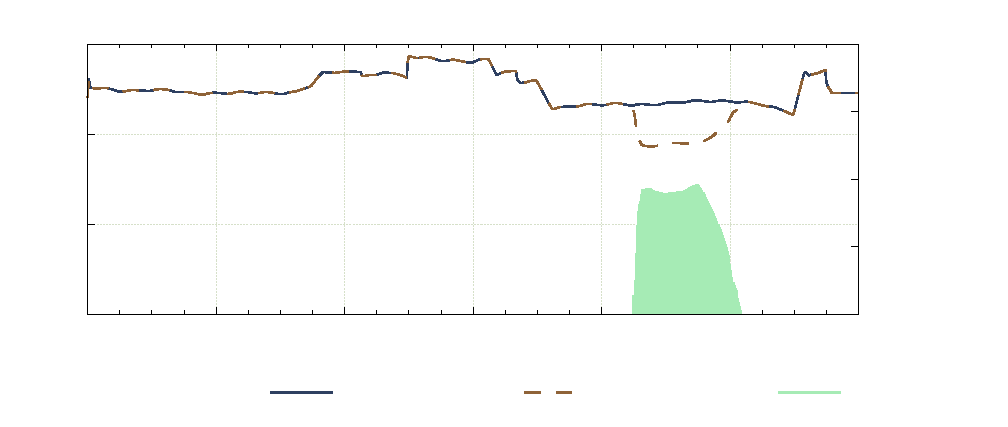
\includegraphics[trim=0 0 0.1cm 0, clip]{Graphs/4/BeetResults/ValveSetpoints/ValveSetpoints}}}%
    \gplfronttext
  \end{picture}%
\endgroup

	\caption{Power savings}
	\label{fig: Control Valve Results Beatrix}
\end{figure}
\subsection{Validation of results}
\begin{figure}[h!]
	\centering
	% GNUPLOT: LaTeX picture with Postscript
\begingroup
  \makeatletter
  \providecommand\color[2][]{%
    \GenericError{(gnuplot) \space\space\space\@spaces}{%
      Package color not loaded in conjunction with
      terminal option `colourtext'%
    }{See the gnuplot documentation for explanation.%
    }{Either use 'blacktext' in gnuplot or load the package
      color.sty in LaTeX.}%
    \renewcommand\color[2][]{}%
  }%
  \providecommand\includegraphics[2][]{%
    \GenericError{(gnuplot) \space\space\space\@spaces}{%
      Package graphicx or graphics not loaded%
    }{See the gnuplot documentation for explanation.%
    }{The gnuplot epslatex terminal needs graphicx.sty or graphics.sty.}%
    \renewcommand\includegraphics[2][]{}%
  }%
  \providecommand\rotatebox[2]{#2}%
  \@ifundefined{ifGPcolor}{%
    \newif\ifGPcolor
    \GPcolortrue
  }{}%
  \@ifundefined{ifGPblacktext}{%
    \newif\ifGPblacktext
    \GPblacktextfalse
  }{}%
  % define a \g@addto@macro without @ in the name:
  \let\gplgaddtomacro\g@addto@macro
  % define empty templates for all commands taking text:
  \gdef\gplbacktext{}%
  \gdef\gplfronttext{}%
  \makeatother
  \ifGPblacktext
    % no textcolor at all
    \def\colorrgb#1{}%
    \def\colorgray#1{}%
  \else
    % gray or color?
    \ifGPcolor
      \def\colorrgb#1{\color[rgb]{#1}}%
      \def\colorgray#1{\color[gray]{#1}}%
      \expandafter\def\csname LTw\endcsname{\color{white}}%
      \expandafter\def\csname LTb\endcsname{\color{black}}%
      \expandafter\def\csname LTa\endcsname{\color{black}}%
      \expandafter\def\csname LT0\endcsname{\color[rgb]{1,0,0}}%
      \expandafter\def\csname LT1\endcsname{\color[rgb]{0,1,0}}%
      \expandafter\def\csname LT2\endcsname{\color[rgb]{0,0,1}}%
      \expandafter\def\csname LT3\endcsname{\color[rgb]{1,0,1}}%
      \expandafter\def\csname LT4\endcsname{\color[rgb]{0,1,1}}%
      \expandafter\def\csname LT5\endcsname{\color[rgb]{1,1,0}}%
      \expandafter\def\csname LT6\endcsname{\color[rgb]{0,0,0}}%
      \expandafter\def\csname LT7\endcsname{\color[rgb]{1,0.3,0}}%
      \expandafter\def\csname LT8\endcsname{\color[rgb]{0.5,0.5,0.5}}%
    \else
      % gray
      \def\colorrgb#1{\color{black}}%
      \def\colorgray#1{\color[gray]{#1}}%
      \expandafter\def\csname LTw\endcsname{\color{white}}%
      \expandafter\def\csname LTb\endcsname{\color{black}}%
      \expandafter\def\csname LTa\endcsname{\color{black}}%
      \expandafter\def\csname LT0\endcsname{\color{black}}%
      \expandafter\def\csname LT1\endcsname{\color{black}}%
      \expandafter\def\csname LT2\endcsname{\color{black}}%
      \expandafter\def\csname LT3\endcsname{\color{black}}%
      \expandafter\def\csname LT4\endcsname{\color{black}}%
      \expandafter\def\csname LT5\endcsname{\color{black}}%
      \expandafter\def\csname LT6\endcsname{\color{black}}%
      \expandafter\def\csname LT7\endcsname{\color{black}}%
      \expandafter\def\csname LT8\endcsname{\color{black}}%
    \fi
  \fi
    \setlength{\unitlength}{0.0500bp}%
    \ifx\gptboxheight\undefined%
      \newlength{\gptboxheight}%
      \newlength{\gptboxwidth}%
      \newsavebox{\gptboxtext}%
    \fi%
    \setlength{\fboxrule}{0.5pt}%
    \setlength{\fboxsep}{1pt}%
\begin{picture}(9360.00,3780.00)%
    \gplgaddtomacro\gplbacktext{%
      \colorrgb{0.00,0.00,0.00}%
      \put(550,924){\makebox(0,0)[r]{\strut{}$0$}}%
      \colorrgb{0.00,0.00,0.00}%
      \put(550,1788){\makebox(0,0)[r]{\strut{}$2$}}%
      \colorrgb{0.00,0.00,0.00}%
      \put(550,2651){\makebox(0,0)[r]{\strut{}$4$}}%
      \colorrgb{0.00,0.00,0.00}%
      \put(550,3515){\makebox(0,0)[r]{\strut{}$6$}}%
      \colorrgb{0.00,0.00,0.00}%
      \put(682,704){\makebox(0,0){\strut{}00:00}}%
      \colorrgb{0.00,0.00,0.00}%
      \put(1915,704){\makebox(0,0){\strut{}04:00}}%
      \colorrgb{0.00,0.00,0.00}%
      \put(3149,704){\makebox(0,0){\strut{}08:00}}%
      \colorrgb{0.00,0.00,0.00}%
      \put(4382,704){\makebox(0,0){\strut{}12:00}}%
      \colorrgb{0.00,0.00,0.00}%
      \put(5615,704){\makebox(0,0){\strut{}16:00}}%
      \colorrgb{0.00,0.00,0.00}%
      \put(6849,704){\makebox(0,0){\strut{}20:00}}%
      \colorrgb{0.00,0.00,0.00}%
      \put(8082,704){\makebox(0,0){\strut{}00:00}}%
      \colorrgb{0.00,0.00,0.00}%
      \put(8214,924){\makebox(0,0)[l]{\strut{}$0$}}%
      \colorrgb{0.00,0.00,0.00}%
      \put(8214,1572){\makebox(0,0)[l]{\strut{}$0.5$}}%
      \colorrgb{0.00,0.00,0.00}%
      \put(8214,2220){\makebox(0,0)[l]{\strut{}$1$}}%
      \colorrgb{0.00,0.00,0.00}%
      \put(8214,2867){\makebox(0,0)[l]{\strut{}$1.5$}}%
      \colorrgb{0.00,0.00,0.00}%
      \put(8214,3515){\makebox(0,0)[l]{\strut{}$2$}}%
    }%
    \gplgaddtomacro\gplfronttext{%
      \csname LTb\endcsname%
      \put(176,2219){\rotatebox{-270}{\makebox(0,0){\strut{}Power $(MW)$}}}%
      \put(8851,2219){\rotatebox{-270}{\makebox(0,0){\strut{}Power Saving $(MW)$}}}%
      \put(4382,374){\makebox(0,0){\strut{}Time of Day}}%
      \csname LTb\endcsname%
      \put(2307,173){\makebox(0,0)[r]{\strut{}Baseline}}%
      \csname LTb\endcsname%
      \put(4746,173){\makebox(0,0)[r]{\strut{}Actual}}%
      \csname LTb\endcsname%
      \put(7185,173){\makebox(0,0)[r]{\strut{}Power saving}}%
    }%
    \gplbacktext
    \put(0,0){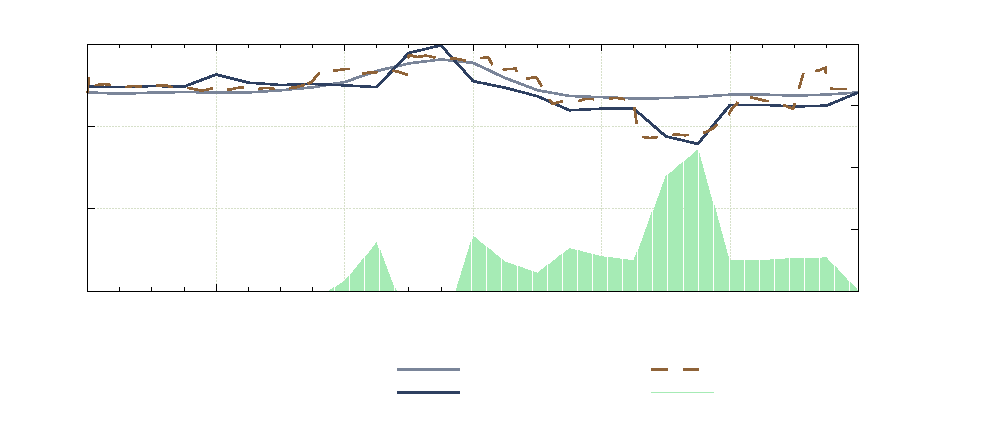
\includegraphics{Graphs/4/BeetValidate/BeetValidate}}%
    \gplfronttext
  \end{picture}%
\endgroup

	\caption{Actual power savings achieved on the system}
	\label{fig: Actual permormance beet}
\end{figure}
\subsection{Summary}
\newpage
\section{Case study B \tiny{\color{blue}(Kusasalethu)}}

	\subsection{System investigation}
	Case study B is another large South African gold mine. The mine utilises five compressors supply compressed air to various surface and underground operations. An investigation was performed to gather the data and information required to build a simulation model of the network.
	\par 
	A basic air distribution layout was obtained, as shown in Figure \ref{fig: KUS Air layout}.  The figure indicates available meters and instrumentation as well as typical airflow splits to various sections and levels of the mine.
	\par 

	\begin{figure}[h!]
		\centering
		\fbox{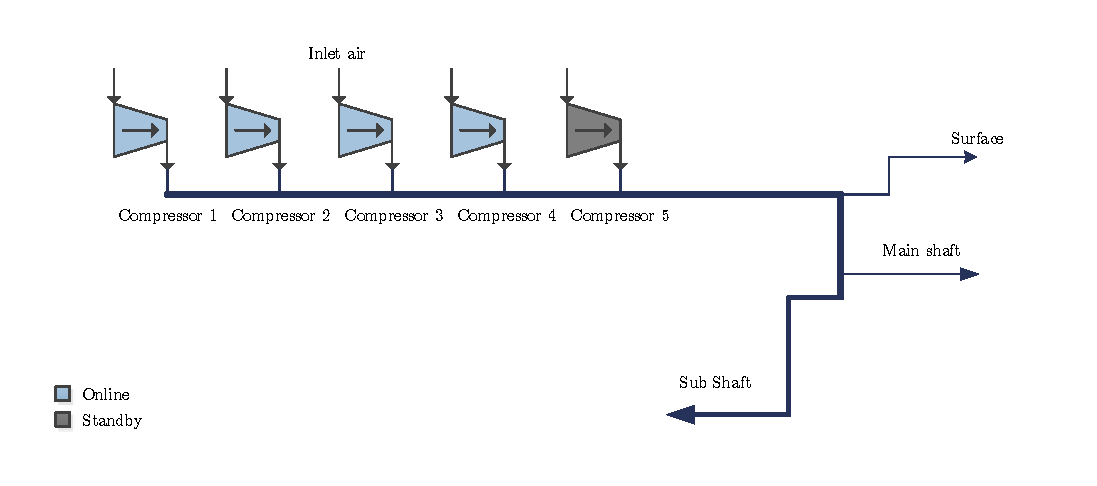
\includegraphics[trim =0cm 0.6cm 0cm 0.6cm,width=\textwidth]{Graphs/4/KUSLayout1/KUSLayout1.pdf}}
		\caption{Basic layout of the compressed air network.}
		\label{fig: KUS Air layout}
	\end{figure}
 To understand the operation of the system, schedules and set-points as well as critical limits such as minimum and maximum pressures were obtained from various personal and from the \gls{scada}. Important data parameters such as Powers, pressures, flows, etc. for the system was gathered from the \gls{scada} and other data sources. This data will be used to develop and calibrate the simulation model
\par 
		
	An in-depth investigation was performed on the significant mining levels to map the locations of mining cross-sections, refuge bays, major leaks and other compressed air consumers on each level as well as measure the usages. An example of a resultant schematic from the underground investigation is shown in Figure \ref{fig: KUS Underground level layout}
	
%	\begin{figure}[h]
%		\centering
%		\fbox{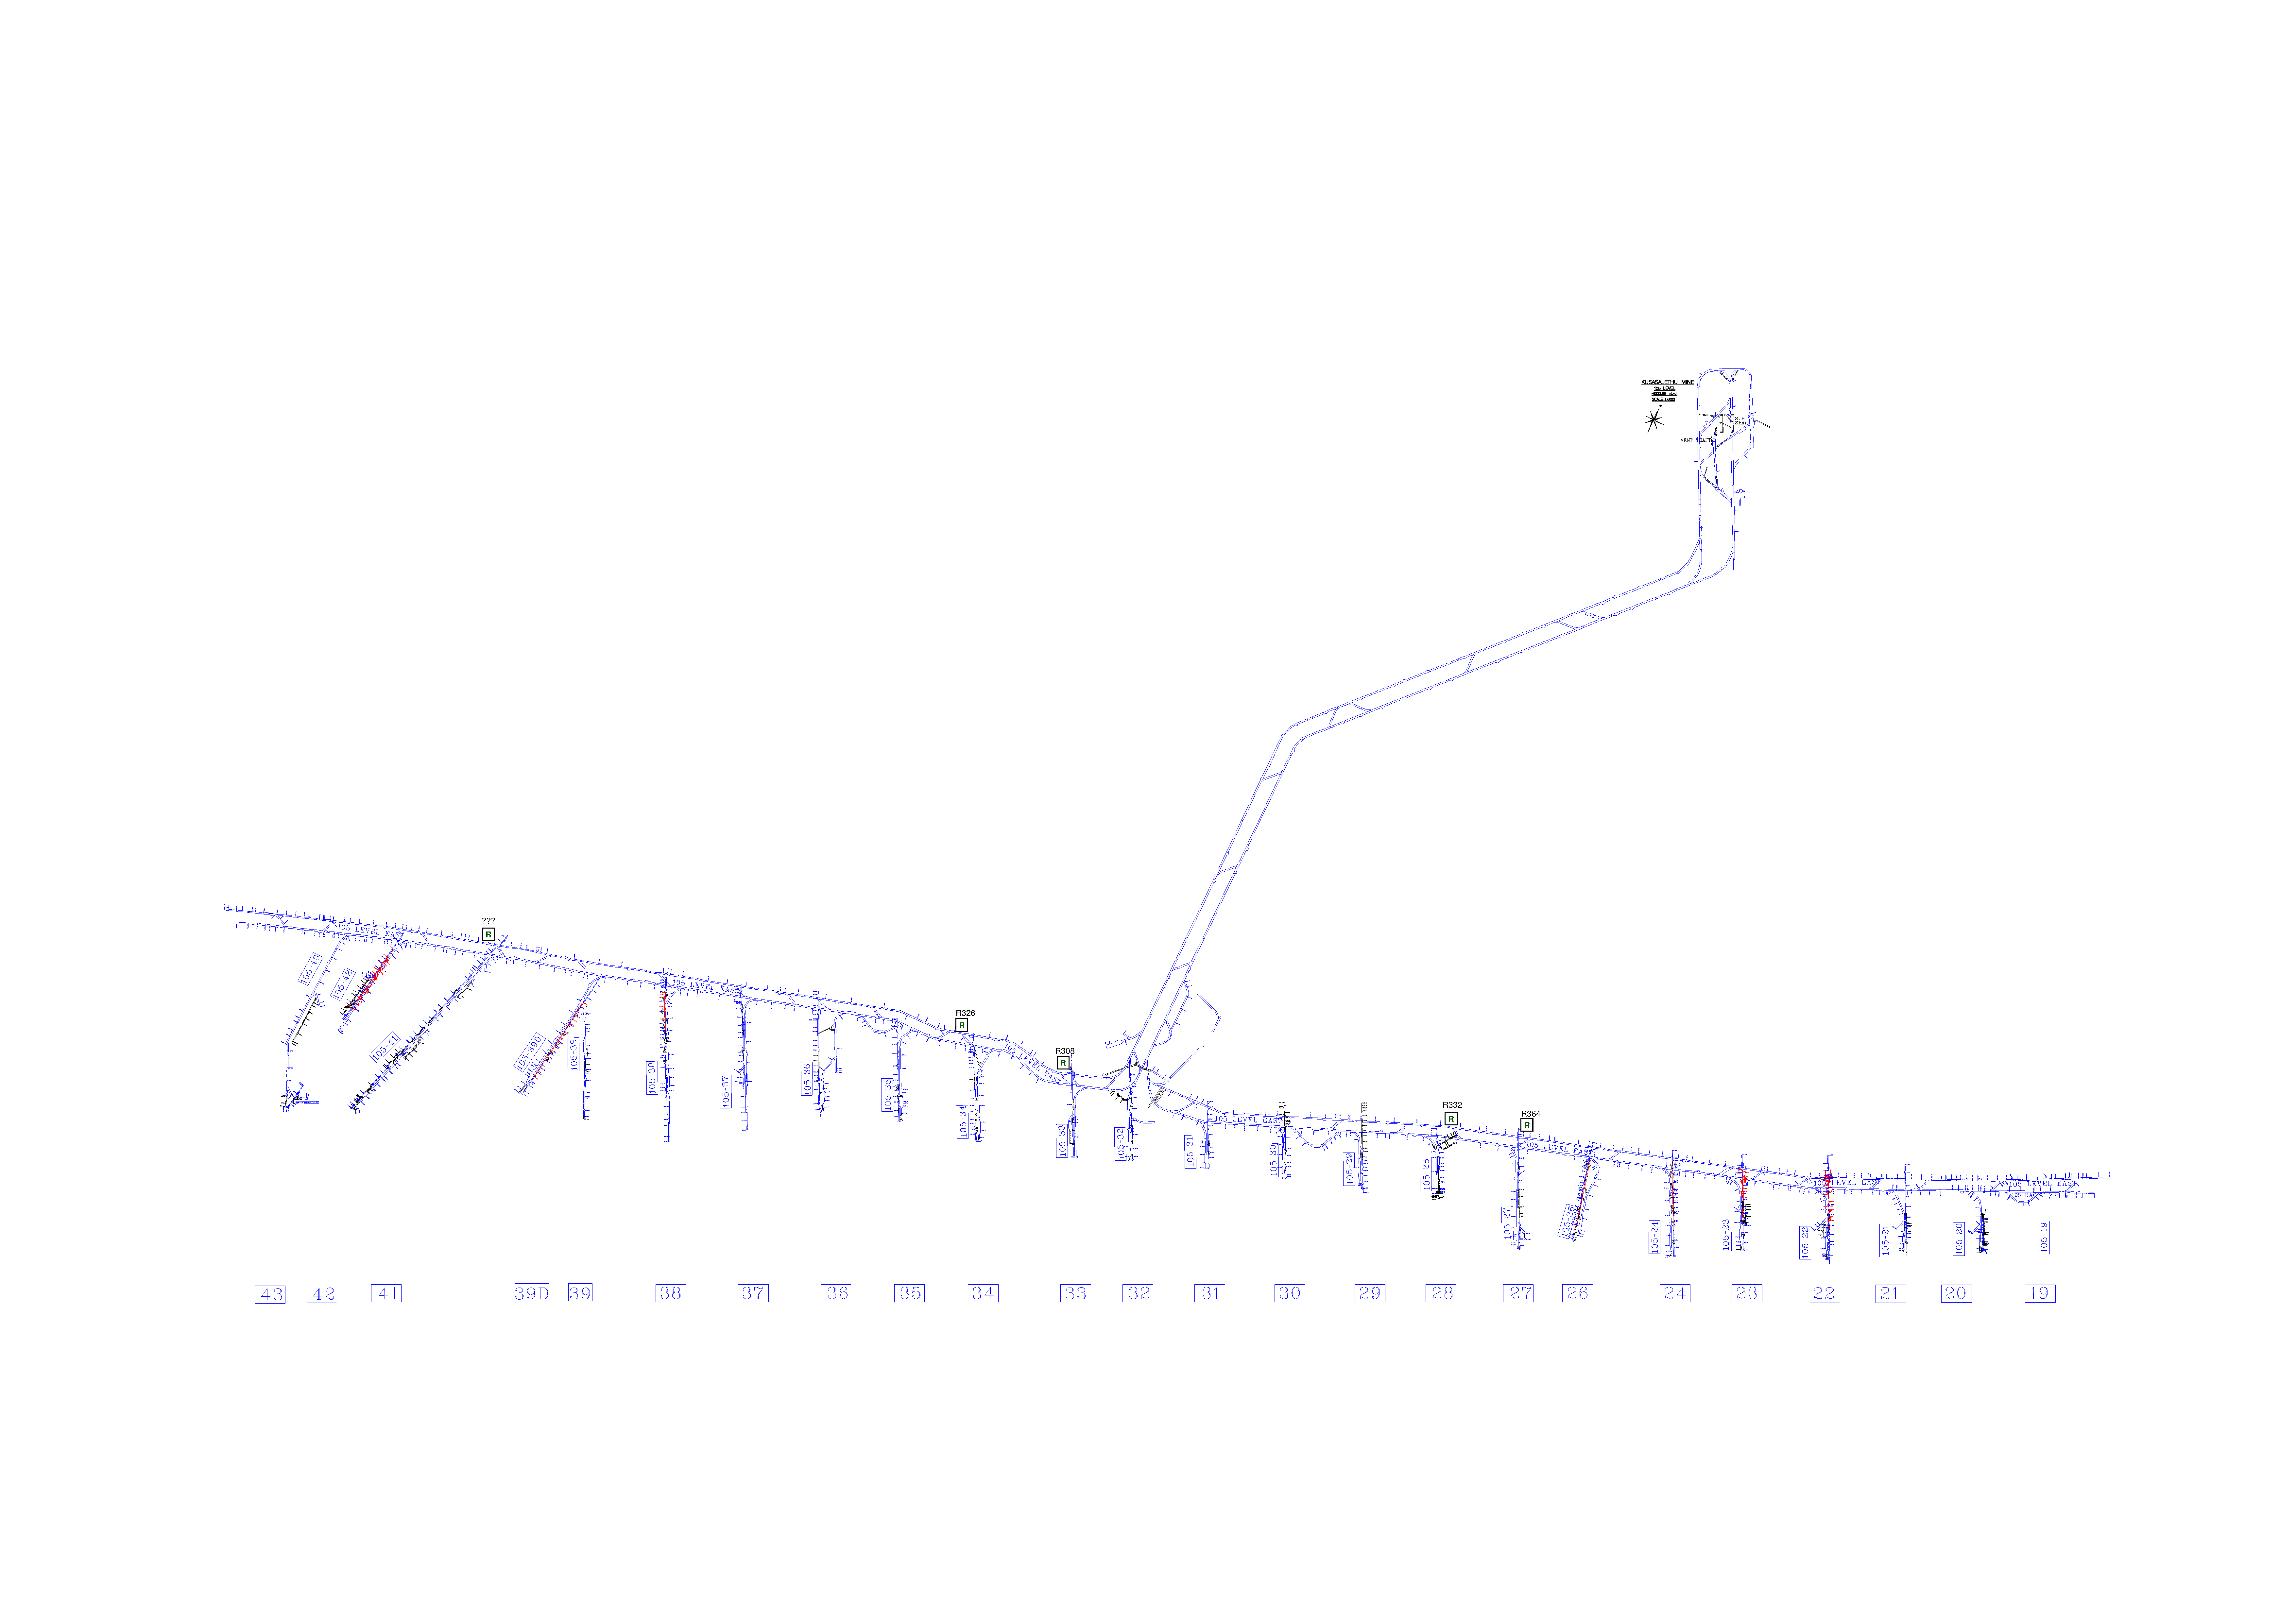
\includegraphics[trim =9cm 12cm 9cm 15cm,angle=90, height=\textheight]{Graphs/4/LevelLayout/105L.pdf}}
%		\caption{Underground level layout.}
%		\label{fig: KUS Underground level layout}
%	\end{figure}	
	\subsection{Model development}
	
	Using the data obtained from the investigation of the system, a  simulation model was developed in software. The modelling methodology described in Chapter 3 was then utilised to develop a model for the system. The entire model is shown in Appendix \ref{ASchematics} Figure \ref{fig: KUS Baseline model}. The model parameters were then calibrated to match the actual data from the mine.
	
	\subsubsection{Verification of baseline simulation}
	Using the verification methodology, the simulation model was performed by comparing the simulation outputs to actual measured values. To simplify the model, the actual measured pressure is temporarily used as set points for the compressors. This ensured that the pressure in the network is identical to that of the actual measured system as shown in Figure \ref{fig: Verification Pressure kusasalethu}.
	
	\par 
	
	\begin{figure}[h]
		\centering
		% GNUPLOT: LaTeX picture with Postscript
\begingroup
  \makeatletter
  \providecommand\color[2][]{%
    \GenericError{(gnuplot) \space\space\space\@spaces}{%
      Package color not loaded in conjunction with
      terminal option `colourtext'%
    }{See the gnuplot documentation for explanation.%
    }{Either use 'blacktext' in gnuplot or load the package
      color.sty in LaTeX.}%
    \renewcommand\color[2][]{}%
  }%
  \providecommand\includegraphics[2][]{%
    \GenericError{(gnuplot) \space\space\space\@spaces}{%
      Package graphicx or graphics not loaded%
    }{See the gnuplot documentation for explanation.%
    }{The gnuplot epslatex terminal needs graphicx.sty or graphics.sty.}%
    \renewcommand\includegraphics[2][]{}%
  }%
  \providecommand\rotatebox[2]{#2}%
  \@ifundefined{ifGPcolor}{%
    \newif\ifGPcolor
    \GPcolortrue
  }{}%
  \@ifundefined{ifGPblacktext}{%
    \newif\ifGPblacktext
    \GPblacktextfalse
  }{}%
  % define a \g@addto@macro without @ in the name:
  \let\gplgaddtomacro\g@addto@macro
  % define empty templates for all commands taking text:
  \gdef\gplbacktext{}%
  \gdef\gplfronttext{}%
  \makeatother
  \ifGPblacktext
    % no textcolor at all
    \def\colorrgb#1{}%
    \def\colorgray#1{}%
  \else
    % gray or color?
    \ifGPcolor
      \def\colorrgb#1{\color[rgb]{#1}}%
      \def\colorgray#1{\color[gray]{#1}}%
      \expandafter\def\csname LTw\endcsname{\color{white}}%
      \expandafter\def\csname LTb\endcsname{\color{black}}%
      \expandafter\def\csname LTa\endcsname{\color{black}}%
      \expandafter\def\csname LT0\endcsname{\color[rgb]{1,0,0}}%
      \expandafter\def\csname LT1\endcsname{\color[rgb]{0,1,0}}%
      \expandafter\def\csname LT2\endcsname{\color[rgb]{0,0,1}}%
      \expandafter\def\csname LT3\endcsname{\color[rgb]{1,0,1}}%
      \expandafter\def\csname LT4\endcsname{\color[rgb]{0,1,1}}%
      \expandafter\def\csname LT5\endcsname{\color[rgb]{1,1,0}}%
      \expandafter\def\csname LT6\endcsname{\color[rgb]{0,0,0}}%
      \expandafter\def\csname LT7\endcsname{\color[rgb]{1,0.3,0}}%
      \expandafter\def\csname LT8\endcsname{\color[rgb]{0.5,0.5,0.5}}%
    \else
      % gray
      \def\colorrgb#1{\color{black}}%
      \def\colorgray#1{\color[gray]{#1}}%
      \expandafter\def\csname LTw\endcsname{\color{white}}%
      \expandafter\def\csname LTb\endcsname{\color{black}}%
      \expandafter\def\csname LTa\endcsname{\color{black}}%
      \expandafter\def\csname LT0\endcsname{\color{black}}%
      \expandafter\def\csname LT1\endcsname{\color{black}}%
      \expandafter\def\csname LT2\endcsname{\color{black}}%
      \expandafter\def\csname LT3\endcsname{\color{black}}%
      \expandafter\def\csname LT4\endcsname{\color{black}}%
      \expandafter\def\csname LT5\endcsname{\color{black}}%
      \expandafter\def\csname LT6\endcsname{\color{black}}%
      \expandafter\def\csname LT7\endcsname{\color{black}}%
      \expandafter\def\csname LT8\endcsname{\color{black}}%
    \fi
  \fi
    \setlength{\unitlength}{0.0500bp}%
    \ifx\gptboxheight\undefined%
      \newlength{\gptboxheight}%
      \newlength{\gptboxwidth}%
      \newsavebox{\gptboxtext}%
    \fi%
    \setlength{\fboxrule}{0.5pt}%
    \setlength{\fboxsep}{1pt}%
\begin{picture}(9360.00,2772.00)%
    \gplgaddtomacro\gplbacktext{%
      \colorrgb{0.00,0.00,0.00}%
      \put(814,924){\makebox(0,0)[r]{\strut{}$300$}}%
      \colorrgb{0.00,0.00,0.00}%
      \put(814,1452){\makebox(0,0)[r]{\strut{}$350$}}%
      \colorrgb{0.00,0.00,0.00}%
      \put(814,1979){\makebox(0,0)[r]{\strut{}$400$}}%
      \colorrgb{0.00,0.00,0.00}%
      \put(814,2507){\makebox(0,0)[r]{\strut{}$450$}}%
      \colorrgb{0.00,0.00,0.00}%
      \put(946,704){\makebox(0,0){\strut{}00:00}}%
      \colorrgb{0.00,0.00,0.00}%
      \put(2157,704){\makebox(0,0){\strut{}04:00}}%
      \colorrgb{0.00,0.00,0.00}%
      \put(3369,704){\makebox(0,0){\strut{}08:00}}%
      \colorrgb{0.00,0.00,0.00}%
      \put(4580,704){\makebox(0,0){\strut{}12:00}}%
      \colorrgb{0.00,0.00,0.00}%
      \put(5791,704){\makebox(0,0){\strut{}16:00}}%
      \colorrgb{0.00,0.00,0.00}%
      \put(7003,704){\makebox(0,0){\strut{}20:00}}%
      \colorrgb{0.00,0.00,0.00}%
      \put(8214,704){\makebox(0,0){\strut{}00:00}}%
      \colorrgb{0.00,0.00,0.00}%
      \put(8346,924){\makebox(0,0)[l]{\strut{}$0$}}%
      \colorrgb{0.00,0.00,0.00}%
      \put(8346,1557){\makebox(0,0)[l]{\strut{}$10$}}%
      \colorrgb{0.00,0.00,0.00}%
      \put(8346,2190){\makebox(0,0)[l]{\strut{}$20$}}%
    }%
    \gplgaddtomacro\gplfronttext{%
      \csname LTb\endcsname%
      \put(176,1715){\rotatebox{-270}{\makebox(0,0){\strut{}Pressure $(kPa)$}}}%
      \put(8851,1715){\rotatebox{-270}{\makebox(0,0){\strut{}$\% error$}}}%
      \put(4580,374){\makebox(0,0){\strut{}Time of Day}}%
      \csname LTb\endcsname%
      \put(2241,173){\makebox(0,0)[r]{\strut{}Baseline press.}}%
      \csname LTb\endcsname%
      \put(5208,173){\makebox(0,0)[r]{\strut{}Simulated press.}}%
      \csname LTb\endcsname%
      \put(8175,173){\makebox(0,0)[r]{\strut{}Error}}%
    }%
    \gplbacktext
    \put(0,0){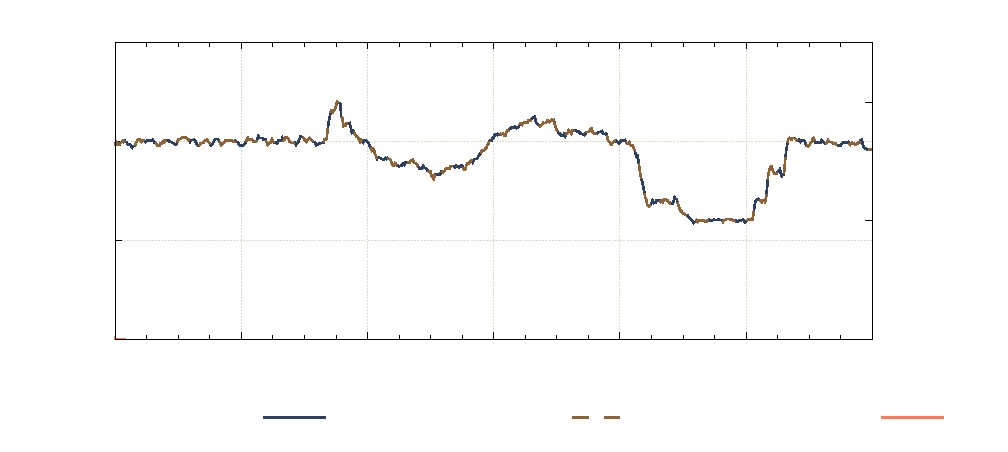
\includegraphics{Graphs/4/KusVerify/Pressure/Pressure}}%
    \gplfronttext
  \end{picture}%
\endgroup

		\caption{Comparing the pressure response of simulation to the actual measured pressure}
		\label{fig: Verification Pressure kusasalethu}
	\end{figure}

 	With the pressure set, the power and air flow outputs for components throughout the model were compared with their relative actual values. Figure \ref{fig: Verification Power kusasalethu} shows the comparison of the total power and flow of the system with the actual measure values for that same period. The accuracy for these parameters compared to the real system was $98.7 \%$ and $99.0 \%$ respectively. This was regarded as acceptable accuracy. 
 
	\begin{figure}[h]
		\centering
		% GNUPLOT: LaTeX picture with Postscript
\begingroup
  \makeatletter
  \providecommand\color[2][]{%
    \GenericError{(gnuplot) \space\space\space\@spaces}{%
      Package color not loaded in conjunction with
      terminal option `colourtext'%
    }{See the gnuplot documentation for explanation.%
    }{Either use 'blacktext' in gnuplot or load the package
      color.sty in LaTeX.}%
    \renewcommand\color[2][]{}%
  }%
  \providecommand\includegraphics[2][]{%
    \GenericError{(gnuplot) \space\space\space\@spaces}{%
      Package graphicx or graphics not loaded%
    }{See the gnuplot documentation for explanation.%
    }{The gnuplot epslatex terminal needs graphicx.sty or graphics.sty.}%
    \renewcommand\includegraphics[2][]{}%
  }%
  \providecommand\rotatebox[2]{#2}%
  \@ifundefined{ifGPcolor}{%
    \newif\ifGPcolor
    \GPcolortrue
  }{}%
  \@ifundefined{ifGPblacktext}{%
    \newif\ifGPblacktext
    \GPblacktextfalse
  }{}%
  % define a \g@addto@macro without @ in the name:
  \let\gplgaddtomacro\g@addto@macro
  % define empty templates for all commands taking text:
  \gdef\gplbacktext{}%
  \gdef\gplfronttext{}%
  \makeatother
  \ifGPblacktext
    % no textcolor at all
    \def\colorrgb#1{}%
    \def\colorgray#1{}%
  \else
    % gray or color?
    \ifGPcolor
      \def\colorrgb#1{\color[rgb]{#1}}%
      \def\colorgray#1{\color[gray]{#1}}%
      \expandafter\def\csname LTw\endcsname{\color{white}}%
      \expandafter\def\csname LTb\endcsname{\color{black}}%
      \expandafter\def\csname LTa\endcsname{\color{black}}%
      \expandafter\def\csname LT0\endcsname{\color[rgb]{1,0,0}}%
      \expandafter\def\csname LT1\endcsname{\color[rgb]{0,1,0}}%
      \expandafter\def\csname LT2\endcsname{\color[rgb]{0,0,1}}%
      \expandafter\def\csname LT3\endcsname{\color[rgb]{1,0,1}}%
      \expandafter\def\csname LT4\endcsname{\color[rgb]{0,1,1}}%
      \expandafter\def\csname LT5\endcsname{\color[rgb]{1,1,0}}%
      \expandafter\def\csname LT6\endcsname{\color[rgb]{0,0,0}}%
      \expandafter\def\csname LT7\endcsname{\color[rgb]{1,0.3,0}}%
      \expandafter\def\csname LT8\endcsname{\color[rgb]{0.5,0.5,0.5}}%
    \else
      % gray
      \def\colorrgb#1{\color{black}}%
      \def\colorgray#1{\color[gray]{#1}}%
      \expandafter\def\csname LTw\endcsname{\color{white}}%
      \expandafter\def\csname LTb\endcsname{\color{black}}%
      \expandafter\def\csname LTa\endcsname{\color{black}}%
      \expandafter\def\csname LT0\endcsname{\color{black}}%
      \expandafter\def\csname LT1\endcsname{\color{black}}%
      \expandafter\def\csname LT2\endcsname{\color{black}}%
      \expandafter\def\csname LT3\endcsname{\color{black}}%
      \expandafter\def\csname LT4\endcsname{\color{black}}%
      \expandafter\def\csname LT5\endcsname{\color{black}}%
      \expandafter\def\csname LT6\endcsname{\color{black}}%
      \expandafter\def\csname LT7\endcsname{\color{black}}%
      \expandafter\def\csname LT8\endcsname{\color{black}}%
    \fi
  \fi
    \setlength{\unitlength}{0.0500bp}%
    \ifx\gptboxheight\undefined%
      \newlength{\gptboxheight}%
      \newlength{\gptboxwidth}%
      \newsavebox{\gptboxtext}%
    \fi%
    \setlength{\fboxrule}{0.5pt}%
    \setlength{\fboxsep}{1pt}%
\begin{picture}(9360.00,3276.00)%
    \gplgaddtomacro\gplbacktext{%
      \colorrgb{0.00,0.00,0.00}%
      \put(682,924){\makebox(0,0)[r]{\strut{}$30$}}%
      \colorrgb{0.00,0.00,0.00}%
      \put(682,1967){\makebox(0,0)[r]{\strut{}$40$}}%
      \colorrgb{0.00,0.00,0.00}%
      \put(682,3011){\makebox(0,0)[r]{\strut{}$50$}}%
      \colorrgb{0.00,0.00,0.00}%
      \put(814,704){\makebox(0,0){\strut{}00:00}}%
      \colorrgb{0.00,0.00,0.00}%
      \put(2047,704){\makebox(0,0){\strut{}04:00}}%
      \colorrgb{0.00,0.00,0.00}%
      \put(3281,704){\makebox(0,0){\strut{}08:00}}%
      \colorrgb{0.00,0.00,0.00}%
      \put(4514,704){\makebox(0,0){\strut{}12:00}}%
      \colorrgb{0.00,0.00,0.00}%
      \put(5747,704){\makebox(0,0){\strut{}16:00}}%
      \colorrgb{0.00,0.00,0.00}%
      \put(6981,704){\makebox(0,0){\strut{}20:00}}%
      \colorrgb{0.00,0.00,0.00}%
      \put(8214,704){\makebox(0,0){\strut{}00:00}}%
      \colorrgb{0.00,0.00,0.00}%
      \put(8346,924){\makebox(0,0)[l]{\strut{}$0$}}%
      \colorrgb{0.00,0.00,0.00}%
      \put(8346,1759){\makebox(0,0)[l]{\strut{}$10$}}%
      \colorrgb{0.00,0.00,0.00}%
      \put(8346,2594){\makebox(0,0)[l]{\strut{}$20$}}%
    }%
    \gplgaddtomacro\gplfronttext{%
      \csname LTb\endcsname%
      \put(176,1967){\rotatebox{-270}{\makebox(0,0){\strut{}flow $(kg/s)$}}}%
      \put(8851,1967){\rotatebox{-270}{\makebox(0,0){\strut{}$\% error$}}}%
      \put(4514,374){\makebox(0,0){\strut{}Time of Day}}%
      \csname LTb\endcsname%
      \put(2307,173){\makebox(0,0)[r]{\strut{}Baseline flow}}%
      \csname LTb\endcsname%
      \put(5010,173){\makebox(0,0)[r]{\strut{}Simulated flow}}%
      \csname LTb\endcsname%
      \put(7713,173){\makebox(0,0)[r]{\strut{}Error}}%
    }%
    \gplbacktext
    \put(0,0){\fbox{
\includegraphics[trim=0 0 0.1cm 0, clip]{Graphs/4/KusVerify/Flow/Flow}}}%
    \gplfronttext
  \end{picture}%
\endgroup

		(a)\\
		% GNUPLOT: LaTeX picture with Postscript
\begingroup
  \makeatletter
  \providecommand\color[2][]{%
    \GenericError{(gnuplot) \space\space\space\@spaces}{%
      Package color not loaded in conjunction with
      terminal option `colourtext'%
    }{See the gnuplot documentation for explanation.%
    }{Either use 'blacktext' in gnuplot or load the package
      color.sty in LaTeX.}%
    \renewcommand\color[2][]{}%
  }%
  \providecommand\includegraphics[2][]{%
    \GenericError{(gnuplot) \space\space\space\@spaces}{%
      Package graphicx or graphics not loaded%
    }{See the gnuplot documentation for explanation.%
    }{The gnuplot epslatex terminal needs graphicx.sty or graphics.sty.}%
    \renewcommand\includegraphics[2][]{}%
  }%
  \providecommand\rotatebox[2]{#2}%
  \@ifundefined{ifGPcolor}{%
    \newif\ifGPcolor
    \GPcolortrue
  }{}%
  \@ifundefined{ifGPblacktext}{%
    \newif\ifGPblacktext
    \GPblacktextfalse
  }{}%
  % define a \g@addto@macro without @ in the name:
  \let\gplgaddtomacro\g@addto@macro
  % define empty templates for all commands taking text:
  \gdef\gplbacktext{}%
  \gdef\gplfronttext{}%
  \makeatother
  \ifGPblacktext
    % no textcolor at all
    \def\colorrgb#1{}%
    \def\colorgray#1{}%
  \else
    % gray or color?
    \ifGPcolor
      \def\colorrgb#1{\color[rgb]{#1}}%
      \def\colorgray#1{\color[gray]{#1}}%
      \expandafter\def\csname LTw\endcsname{\color{white}}%
      \expandafter\def\csname LTb\endcsname{\color{black}}%
      \expandafter\def\csname LTa\endcsname{\color{black}}%
      \expandafter\def\csname LT0\endcsname{\color[rgb]{1,0,0}}%
      \expandafter\def\csname LT1\endcsname{\color[rgb]{0,1,0}}%
      \expandafter\def\csname LT2\endcsname{\color[rgb]{0,0,1}}%
      \expandafter\def\csname LT3\endcsname{\color[rgb]{1,0,1}}%
      \expandafter\def\csname LT4\endcsname{\color[rgb]{0,1,1}}%
      \expandafter\def\csname LT5\endcsname{\color[rgb]{1,1,0}}%
      \expandafter\def\csname LT6\endcsname{\color[rgb]{0,0,0}}%
      \expandafter\def\csname LT7\endcsname{\color[rgb]{1,0.3,0}}%
      \expandafter\def\csname LT8\endcsname{\color[rgb]{0.5,0.5,0.5}}%
    \else
      % gray
      \def\colorrgb#1{\color{black}}%
      \def\colorgray#1{\color[gray]{#1}}%
      \expandafter\def\csname LTw\endcsname{\color{white}}%
      \expandafter\def\csname LTb\endcsname{\color{black}}%
      \expandafter\def\csname LTa\endcsname{\color{black}}%
      \expandafter\def\csname LT0\endcsname{\color{black}}%
      \expandafter\def\csname LT1\endcsname{\color{black}}%
      \expandafter\def\csname LT2\endcsname{\color{black}}%
      \expandafter\def\csname LT3\endcsname{\color{black}}%
      \expandafter\def\csname LT4\endcsname{\color{black}}%
      \expandafter\def\csname LT5\endcsname{\color{black}}%
      \expandafter\def\csname LT6\endcsname{\color{black}}%
      \expandafter\def\csname LT7\endcsname{\color{black}}%
      \expandafter\def\csname LT8\endcsname{\color{black}}%
    \fi
  \fi
    \setlength{\unitlength}{0.0500bp}%
    \ifx\gptboxheight\undefined%
      \newlength{\gptboxheight}%
      \newlength{\gptboxwidth}%
      \newsavebox{\gptboxtext}%
    \fi%
    \setlength{\fboxrule}{0.5pt}%
    \setlength{\fboxsep}{1pt}%
\begin{picture}(9360.00,3276.00)%
    \gplgaddtomacro\gplbacktext{%
      \colorrgb{0.00,0.00,0.00}%
      \put(682,924){\makebox(0,0)[r]{\strut{}$8$}}%
      \colorrgb{0.00,0.00,0.00}%
      \put(682,1222){\makebox(0,0)[r]{\strut{}$9$}}%
      \colorrgb{0.00,0.00,0.00}%
      \put(682,1520){\makebox(0,0)[r]{\strut{}$10$}}%
      \colorrgb{0.00,0.00,0.00}%
      \put(682,1818){\makebox(0,0)[r]{\strut{}$11$}}%
      \colorrgb{0.00,0.00,0.00}%
      \put(682,2117){\makebox(0,0)[r]{\strut{}$12$}}%
      \colorrgb{0.00,0.00,0.00}%
      \put(682,2415){\makebox(0,0)[r]{\strut{}$13$}}%
      \colorrgb{0.00,0.00,0.00}%
      \put(682,2713){\makebox(0,0)[r]{\strut{}$14$}}%
      \colorrgb{0.00,0.00,0.00}%
      \put(682,3011){\makebox(0,0)[r]{\strut{}$15$}}%
      \colorrgb{0.00,0.00,0.00}%
      \put(814,704){\makebox(0,0){\strut{}00:00}}%
      \colorrgb{0.00,0.00,0.00}%
      \put(2047,704){\makebox(0,0){\strut{}04:00}}%
      \colorrgb{0.00,0.00,0.00}%
      \put(3281,704){\makebox(0,0){\strut{}08:00}}%
      \colorrgb{0.00,0.00,0.00}%
      \put(4514,704){\makebox(0,0){\strut{}12:00}}%
      \colorrgb{0.00,0.00,0.00}%
      \put(5747,704){\makebox(0,0){\strut{}16:00}}%
      \colorrgb{0.00,0.00,0.00}%
      \put(6981,704){\makebox(0,0){\strut{}20:00}}%
      \colorrgb{0.00,0.00,0.00}%
      \put(8214,704){\makebox(0,0){\strut{}00:00}}%
      \colorrgb{0.00,0.00,0.00}%
      \put(8346,924){\makebox(0,0)[l]{\strut{}$0$}}%
      \colorrgb{0.00,0.00,0.00}%
      \put(8346,1759){\makebox(0,0)[l]{\strut{}$10$}}%
      \colorrgb{0.00,0.00,0.00}%
      \put(8346,2594){\makebox(0,0)[l]{\strut{}$20$}}%
    }%
    \gplgaddtomacro\gplfronttext{%
      \csname LTb\endcsname%
      \put(176,1967){\rotatebox{-270}{\makebox(0,0){\strut{}Power $(MW)$}}}%
      \put(8851,1967){\rotatebox{-270}{\makebox(0,0){\strut{}$\% error$}}}%
      \put(4514,374){\makebox(0,0){\strut{}Time of Day}}%
      \csname LTb\endcsname%
      \put(2241,173){\makebox(0,0)[r]{\strut{}Baseline power}}%
      \csname LTb\endcsname%
      \put(5076,173){\makebox(0,0)[r]{\strut{}Simulated power}}%
      \csname LTb\endcsname%
      \put(7911,173){\makebox(0,0)[r]{\strut{}Error}}%
    }%
    \gplbacktext
    \put(0,0){\fbox{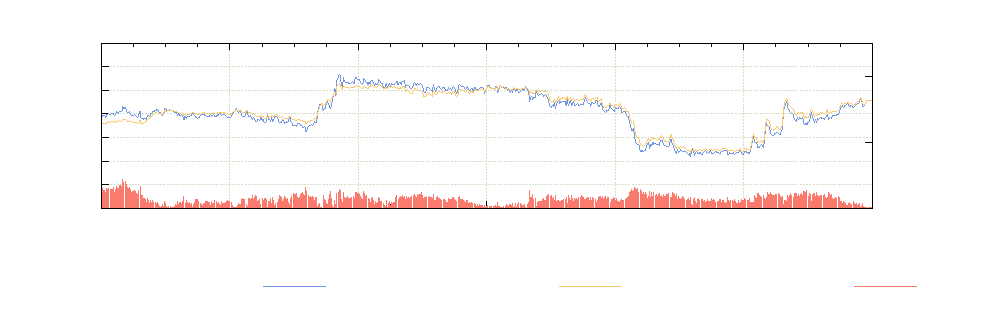
\includegraphics[trim=0 0 0.1cm 0, clip]{Graphs/4/KusVerify/Power/Power}}}%
    \gplfronttext
  \end{picture}%
\endgroup

		(b)\\
		\caption{Verification of the total (a) flow and (b) power of the system using the actual pressure profile.}
		\label{fig: Verification Power kusasalethu}
	\end{figure}

	Once all the power and flow parameters were checked calibrated with minimal error, the system's response to the pressure set-points was checked. The compressor models were replaced with the pressure set-point profile instead of the measured outlet pressure profile. The simulated outlet pressure was then compared to the actual measured outlet, this is shown in Figure \ref{fig: Verification Pressure kusasalethu Setpoint}.

	\begin{figure}[h]
		\centering
		% GNUPLOT: LaTeX picture with Postscript
\begingroup
  \makeatletter
  \providecommand\color[2][]{%
    \GenericError{(gnuplot) \space\space\space\@spaces}{%
      Package color not loaded in conjunction with
      terminal option `colourtext'%
    }{See the gnuplot documentation for explanation.%
    }{Either use 'blacktext' in gnuplot or load the package
      color.sty in LaTeX.}%
    \renewcommand\color[2][]{}%
  }%
  \providecommand\includegraphics[2][]{%
    \GenericError{(gnuplot) \space\space\space\@spaces}{%
      Package graphicx or graphics not loaded%
    }{See the gnuplot documentation for explanation.%
    }{The gnuplot epslatex terminal needs graphicx.sty or graphics.sty.}%
    \renewcommand\includegraphics[2][]{}%
  }%
  \providecommand\rotatebox[2]{#2}%
  \@ifundefined{ifGPcolor}{%
    \newif\ifGPcolor
    \GPcolortrue
  }{}%
  \@ifundefined{ifGPblacktext}{%
    \newif\ifGPblacktext
    \GPblacktextfalse
  }{}%
  % define a \g@addto@macro without @ in the name:
  \let\gplgaddtomacro\g@addto@macro
  % define empty templates for all commands taking text:
  \gdef\gplbacktext{}%
  \gdef\gplfronttext{}%
  \makeatother
  \ifGPblacktext
    % no textcolor at all
    \def\colorrgb#1{}%
    \def\colorgray#1{}%
  \else
    % gray or color?
    \ifGPcolor
      \def\colorrgb#1{\color[rgb]{#1}}%
      \def\colorgray#1{\color[gray]{#1}}%
      \expandafter\def\csname LTw\endcsname{\color{white}}%
      \expandafter\def\csname LTb\endcsname{\color{black}}%
      \expandafter\def\csname LTa\endcsname{\color{black}}%
      \expandafter\def\csname LT0\endcsname{\color[rgb]{1,0,0}}%
      \expandafter\def\csname LT1\endcsname{\color[rgb]{0,1,0}}%
      \expandafter\def\csname LT2\endcsname{\color[rgb]{0,0,1}}%
      \expandafter\def\csname LT3\endcsname{\color[rgb]{1,0,1}}%
      \expandafter\def\csname LT4\endcsname{\color[rgb]{0,1,1}}%
      \expandafter\def\csname LT5\endcsname{\color[rgb]{1,1,0}}%
      \expandafter\def\csname LT6\endcsname{\color[rgb]{0,0,0}}%
      \expandafter\def\csname LT7\endcsname{\color[rgb]{1,0.3,0}}%
      \expandafter\def\csname LT8\endcsname{\color[rgb]{0.5,0.5,0.5}}%
    \else
      % gray
      \def\colorrgb#1{\color{black}}%
      \def\colorgray#1{\color[gray]{#1}}%
      \expandafter\def\csname LTw\endcsname{\color{white}}%
      \expandafter\def\csname LTb\endcsname{\color{black}}%
      \expandafter\def\csname LTa\endcsname{\color{black}}%
      \expandafter\def\csname LT0\endcsname{\color{black}}%
      \expandafter\def\csname LT1\endcsname{\color{black}}%
      \expandafter\def\csname LT2\endcsname{\color{black}}%
      \expandafter\def\csname LT3\endcsname{\color{black}}%
      \expandafter\def\csname LT4\endcsname{\color{black}}%
      \expandafter\def\csname LT5\endcsname{\color{black}}%
      \expandafter\def\csname LT6\endcsname{\color{black}}%
      \expandafter\def\csname LT7\endcsname{\color{black}}%
      \expandafter\def\csname LT8\endcsname{\color{black}}%
    \fi
  \fi
    \setlength{\unitlength}{0.0500bp}%
    \ifx\gptboxheight\undefined%
      \newlength{\gptboxheight}%
      \newlength{\gptboxwidth}%
      \newsavebox{\gptboxtext}%
    \fi%
    \setlength{\fboxrule}{0.5pt}%
    \setlength{\fboxsep}{1pt}%
\begin{picture}(9360.00,4032.00)%
    \gplgaddtomacro\gplbacktext{%
      \colorrgb{0.00,0.00,0.00}%
      \put(814,1144){\makebox(0,0)[r]{\strut{}$300$}}%
      \colorrgb{0.00,0.00,0.00}%
      \put(814,2018){\makebox(0,0)[r]{\strut{}$350$}}%
      \colorrgb{0.00,0.00,0.00}%
      \put(814,2893){\makebox(0,0)[r]{\strut{}$400$}}%
      \colorrgb{0.00,0.00,0.00}%
      \put(814,3767){\makebox(0,0)[r]{\strut{}$450$}}%
      \colorrgb{0.00,0.00,0.00}%
      \put(946,924){\makebox(0,0){\strut{}00:00}}%
      \colorrgb{0.00,0.00,0.00}%
      \put(2157,924){\makebox(0,0){\strut{}04:00}}%
      \colorrgb{0.00,0.00,0.00}%
      \put(3369,924){\makebox(0,0){\strut{}08:00}}%
      \colorrgb{0.00,0.00,0.00}%
      \put(4580,924){\makebox(0,0){\strut{}12:00}}%
      \colorrgb{0.00,0.00,0.00}%
      \put(5791,924){\makebox(0,0){\strut{}16:00}}%
      \colorrgb{0.00,0.00,0.00}%
      \put(7003,924){\makebox(0,0){\strut{}20:00}}%
      \colorrgb{0.00,0.00,0.00}%
      \put(8214,924){\makebox(0,0){\strut{}00:00}}%
      \colorrgb{0.00,0.00,0.00}%
      \put(8346,1144){\makebox(0,0)[l]{\strut{}$0$}}%
      \colorrgb{0.00,0.00,0.00}%
      \put(8346,2193){\makebox(0,0)[l]{\strut{}$10$}}%
      \colorrgb{0.00,0.00,0.00}%
      \put(8346,3242){\makebox(0,0)[l]{\strut{}$20$}}%
    }%
    \gplgaddtomacro\gplfronttext{%
      \csname LTb\endcsname%
      \put(176,2455){\rotatebox{-270}{\makebox(0,0){\strut{}Pressure $(kPa)$}}}%
      \put(8851,2455){\rotatebox{-270}{\makebox(0,0){\strut{}$\% error$}}}%
      \put(4580,594){\makebox(0,0){\strut{}Time of Day}}%
      \csname LTb\endcsname%
      \put(3725,393){\makebox(0,0)[r]{\strut{}Actual}}%
      \csname LTb\endcsname%
      \put(3725,173){\makebox(0,0)[r]{\strut{}Simulation.}}%
      \csname LTb\endcsname%
      \put(6032,393){\makebox(0,0)[r]{\strut{}Set-point}}%
      \csname LTb\endcsname%
      \put(5900,173){\makebox(0,0)[r]{\strut{}Rel. Error}}%
    }%
    \gplbacktext
    \put(0,0){\fbox{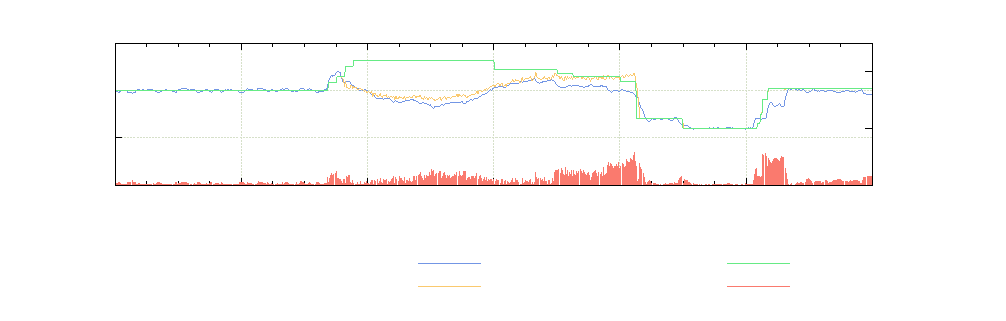
\includegraphics[trim=0 0 0.1cm 0, clip]{Graphs/4/KusVerify/Pressure2/Pressure2}}}%
    \gplfronttext
  \end{picture}%
\endgroup

		\caption{Verifying the Pressure response of the system give the pressure set points as inputs}
		\label{fig: Verification Pressure kusasalethu Setpoint}
	\end{figure}
	\subsection{Scenario 1. Refuge bay optimisation}
	From investigations that were conducted on the mines compressed system, unnecessary refuge bay leaks were identified as a significant inefficiency that can be reduced. A test on a single mining level was performed to  measure the potential flow saving of reducing refuge bay leaks. The test showed that a reduction refuge bay leaks, by closing the valves would lead to a air saving of $0.05$ $kg/s$ per refuge bay at typical operational pressures. This measurement was conservative as not all the refuge bays on the level could be closed for the test. 
	\par 
	Extending these tests to include the rest of the mining sections was not practical due to the size of the mine and high resourse requirement . Therefore, the benefits bay could not accurately be determined from practical tests. Using simulation the typical operation with can be accurately compare with the intervention scenario to quantify the potential financial and operational benefits throughout a given period.
	\par
	The simulation model detail was selected to recreate the scenario within 2\% error. To model auto-compression, the depth of each compressed air component was included into the simulation. Using the per-level layouts obtained from the investigation the location of refuge bay components were identified. Refuge bay leak components were then added to the simulation to replicate the measured leak from each refuge bay. These leaks were modelled as flow demands using the data from the initial refuge bay tests. The overall mass flow of the system was maintained to keap the model accurate. The simulation was verified with an accuracy of 98\% using actual data from the mine. The full simulation process flow diagram is shown in Figure \ref{fig: Refuge bay layout} in Appendix \ref{Schematics}.
	\par 
	
	\begin{figure}[h]
		\centering
		% GNUPLOT: LaTeX picture with Postscript
\begingroup
  \makeatletter
  \providecommand\color[2][]{%
    \GenericError{(gnuplot) \space\space\space\@spaces}{%
      Package color not loaded in conjunction with
      terminal option `colourtext'%
    }{See the gnuplot documentation for explanation.%
    }{Either use 'blacktext' in gnuplot or load the package
      color.sty in LaTeX.}%
    \renewcommand\color[2][]{}%
  }%
  \providecommand\includegraphics[2][]{%
    \GenericError{(gnuplot) \space\space\space\@spaces}{%
      Package graphicx or graphics not loaded%
    }{See the gnuplot documentation for explanation.%
    }{The gnuplot epslatex terminal needs graphicx.sty or graphics.sty.}%
    \renewcommand\includegraphics[2][]{}%
  }%
  \providecommand\rotatebox[2]{#2}%
  \@ifundefined{ifGPcolor}{%
    \newif\ifGPcolor
    \GPcolortrue
  }{}%
  \@ifundefined{ifGPblacktext}{%
    \newif\ifGPblacktext
    \GPblacktextfalse
  }{}%
  % define a \g@addto@macro without @ in the name:
  \let\gplgaddtomacro\g@addto@macro
  % define empty templates for all commands taking text:
  \gdef\gplbacktext{}%
  \gdef\gplfronttext{}%
  \makeatother
  \ifGPblacktext
    % no textcolor at all
    \def\colorrgb#1{}%
    \def\colorgray#1{}%
  \else
    % gray or color?
    \ifGPcolor
      \def\colorrgb#1{\color[rgb]{#1}}%
      \def\colorgray#1{\color[gray]{#1}}%
      \expandafter\def\csname LTw\endcsname{\color{white}}%
      \expandafter\def\csname LTb\endcsname{\color{black}}%
      \expandafter\def\csname LTa\endcsname{\color{black}}%
      \expandafter\def\csname LT0\endcsname{\color[rgb]{1,0,0}}%
      \expandafter\def\csname LT1\endcsname{\color[rgb]{0,1,0}}%
      \expandafter\def\csname LT2\endcsname{\color[rgb]{0,0,1}}%
      \expandafter\def\csname LT3\endcsname{\color[rgb]{1,0,1}}%
      \expandafter\def\csname LT4\endcsname{\color[rgb]{0,1,1}}%
      \expandafter\def\csname LT5\endcsname{\color[rgb]{1,1,0}}%
      \expandafter\def\csname LT6\endcsname{\color[rgb]{0,0,0}}%
      \expandafter\def\csname LT7\endcsname{\color[rgb]{1,0.3,0}}%
      \expandafter\def\csname LT8\endcsname{\color[rgb]{0.5,0.5,0.5}}%
    \else
      % gray
      \def\colorrgb#1{\color{black}}%
      \def\colorgray#1{\color[gray]{#1}}%
      \expandafter\def\csname LTw\endcsname{\color{white}}%
      \expandafter\def\csname LTb\endcsname{\color{black}}%
      \expandafter\def\csname LTa\endcsname{\color{black}}%
      \expandafter\def\csname LT0\endcsname{\color{black}}%
      \expandafter\def\csname LT1\endcsname{\color{black}}%
      \expandafter\def\csname LT2\endcsname{\color{black}}%
      \expandafter\def\csname LT3\endcsname{\color{black}}%
      \expandafter\def\csname LT4\endcsname{\color{black}}%
      \expandafter\def\csname LT5\endcsname{\color{black}}%
      \expandafter\def\csname LT6\endcsname{\color{black}}%
      \expandafter\def\csname LT7\endcsname{\color{black}}%
      \expandafter\def\csname LT8\endcsname{\color{black}}%
    \fi
  \fi
    \setlength{\unitlength}{0.0500bp}%
    \ifx\gptboxheight\undefined%
      \newlength{\gptboxheight}%
      \newlength{\gptboxwidth}%
      \newsavebox{\gptboxtext}%
    \fi%
    \setlength{\fboxrule}{0.5pt}%
    \setlength{\fboxsep}{1pt}%
\begin{picture}(9360.00,3780.00)%
    \gplgaddtomacro\gplbacktext{%
      \colorrgb{0.00,0.00,0.00}%
      \put(682,924){\makebox(0,0)[r]{\strut{}$0$}}%
      \colorrgb{0.00,0.00,0.00}%
      \put(682,1788){\makebox(0,0)[r]{\strut{}$5$}}%
      \colorrgb{0.00,0.00,0.00}%
      \put(682,2651){\makebox(0,0)[r]{\strut{}$10$}}%
      \colorrgb{0.00,0.00,0.00}%
      \put(682,3515){\makebox(0,0)[r]{\strut{}$15$}}%
      \colorrgb{0.00,0.00,0.00}%
      \put(814,704){\makebox(0,0){\strut{}00:00}}%
      \colorrgb{0.00,0.00,0.00}%
      \put(2172,704){\makebox(0,0){\strut{}04:00}}%
      \colorrgb{0.00,0.00,0.00}%
      \put(3530,704){\makebox(0,0){\strut{}08:00}}%
      \colorrgb{0.00,0.00,0.00}%
      \put(4888,704){\makebox(0,0){\strut{}12:00}}%
      \colorrgb{0.00,0.00,0.00}%
      \put(6246,704){\makebox(0,0){\strut{}16:00}}%
      \colorrgb{0.00,0.00,0.00}%
      \put(7604,704){\makebox(0,0){\strut{}20:00}}%
      \colorrgb{0.00,0.00,0.00}%
      \put(8962,704){\makebox(0,0){\strut{}00:00}}%
    }%
    \gplgaddtomacro\gplfronttext{%
      \csname LTb\endcsname%
      \put(176,2219){\rotatebox{-270}{\makebox(0,0){\strut{}Power $(MW)$}}}%
      \put(4888,374){\makebox(0,0){\strut{}Time of Day}}%
      \csname LTb\endcsname%
      \put(2813,173){\makebox(0,0)[r]{\strut{}Baseline}}%
      \csname LTb\endcsname%
      \put(5252,173){\makebox(0,0)[r]{\strut{}Intervention}}%
      \csname LTb\endcsname%
      \put(7691,173){\makebox(0,0)[r]{\strut{}Power saving}}%
    }%
    \gplbacktext
    \put(0,0){
\includegraphics{Graphs/4/KUSResults/RefugePower/RefugePower}}%
    \gplfronttext
  \end{picture}%
\endgroup

		\caption{The Baseline system power compared to the system power when refuge bay leaks are reduced.}
		\label{fig: RefugeBay Power.}
	\end{figure}   

	\begin{figure}[h]
		\centering
		% GNUPLOT: LaTeX picture with Postscript
\begingroup
  \makeatletter
  \providecommand\color[2][]{%
    \GenericError{(gnuplot) \space\space\space\@spaces}{%
      Package color not loaded in conjunction with
      terminal option `colourtext'%
    }{See the gnuplot documentation for explanation.%
    }{Either use 'blacktext' in gnuplot or load the package
      color.sty in LaTeX.}%
    \renewcommand\color[2][]{}%
  }%
  \providecommand\includegraphics[2][]{%
    \GenericError{(gnuplot) \space\space\space\@spaces}{%
      Package graphicx or graphics not loaded%
    }{See the gnuplot documentation for explanation.%
    }{The gnuplot epslatex terminal needs graphicx.sty or graphics.sty.}%
    \renewcommand\includegraphics[2][]{}%
  }%
  \providecommand\rotatebox[2]{#2}%
  \@ifundefined{ifGPcolor}{%
    \newif\ifGPcolor
    \GPcolortrue
  }{}%
  \@ifundefined{ifGPblacktext}{%
    \newif\ifGPblacktext
    \GPblacktextfalse
  }{}%
  % define a \g@addto@macro without @ in the name:
  \let\gplgaddtomacro\g@addto@macro
  % define empty templates for all commands taking text:
  \gdef\gplbacktext{}%
  \gdef\gplfronttext{}%
  \makeatother
  \ifGPblacktext
    % no textcolor at all
    \def\colorrgb#1{}%
    \def\colorgray#1{}%
  \else
    % gray or color?
    \ifGPcolor
      \def\colorrgb#1{\color[rgb]{#1}}%
      \def\colorgray#1{\color[gray]{#1}}%
      \expandafter\def\csname LTw\endcsname{\color{white}}%
      \expandafter\def\csname LTb\endcsname{\color{black}}%
      \expandafter\def\csname LTa\endcsname{\color{black}}%
      \expandafter\def\csname LT0\endcsname{\color[rgb]{1,0,0}}%
      \expandafter\def\csname LT1\endcsname{\color[rgb]{0,1,0}}%
      \expandafter\def\csname LT2\endcsname{\color[rgb]{0,0,1}}%
      \expandafter\def\csname LT3\endcsname{\color[rgb]{1,0,1}}%
      \expandafter\def\csname LT4\endcsname{\color[rgb]{0,1,1}}%
      \expandafter\def\csname LT5\endcsname{\color[rgb]{1,1,0}}%
      \expandafter\def\csname LT6\endcsname{\color[rgb]{0,0,0}}%
      \expandafter\def\csname LT7\endcsname{\color[rgb]{1,0.3,0}}%
      \expandafter\def\csname LT8\endcsname{\color[rgb]{0.5,0.5,0.5}}%
    \else
      % gray
      \def\colorrgb#1{\color{black}}%
      \def\colorgray#1{\color[gray]{#1}}%
      \expandafter\def\csname LTw\endcsname{\color{white}}%
      \expandafter\def\csname LTb\endcsname{\color{black}}%
      \expandafter\def\csname LTa\endcsname{\color{black}}%
      \expandafter\def\csname LT0\endcsname{\color{black}}%
      \expandafter\def\csname LT1\endcsname{\color{black}}%
      \expandafter\def\csname LT2\endcsname{\color{black}}%
      \expandafter\def\csname LT3\endcsname{\color{black}}%
      \expandafter\def\csname LT4\endcsname{\color{black}}%
      \expandafter\def\csname LT5\endcsname{\color{black}}%
      \expandafter\def\csname LT6\endcsname{\color{black}}%
      \expandafter\def\csname LT7\endcsname{\color{black}}%
      \expandafter\def\csname LT8\endcsname{\color{black}}%
    \fi
  \fi
    \setlength{\unitlength}{0.0500bp}%
    \ifx\gptboxheight\undefined%
      \newlength{\gptboxheight}%
      \newlength{\gptboxwidth}%
      \newsavebox{\gptboxtext}%
    \fi%
    \setlength{\fboxrule}{0.5pt}%
    \setlength{\fboxsep}{1pt}%
\begin{picture}(9360.00,3780.00)%
    \gplgaddtomacro\gplbacktext{%
      \colorrgb{0.00,0.00,0.00}%
      \put(814,1183){\makebox(0,0)[r]{\strut{}$360$}}%
      \colorrgb{0.00,0.00,0.00}%
      \put(814,1701){\makebox(0,0)[r]{\strut{}$380$}}%
      \colorrgb{0.00,0.00,0.00}%
      \put(814,2220){\makebox(0,0)[r]{\strut{}$400$}}%
      \colorrgb{0.00,0.00,0.00}%
      \put(814,2738){\makebox(0,0)[r]{\strut{}$420$}}%
      \colorrgb{0.00,0.00,0.00}%
      \put(814,3256){\makebox(0,0)[r]{\strut{}$440$}}%
      \colorrgb{0.00,0.00,0.00}%
      \put(946,704){\makebox(0,0){\strut{}00:00}}%
      \colorrgb{0.00,0.00,0.00}%
      \put(2282,704){\makebox(0,0){\strut{}04:00}}%
      \colorrgb{0.00,0.00,0.00}%
      \put(3618,704){\makebox(0,0){\strut{}08:00}}%
      \colorrgb{0.00,0.00,0.00}%
      \put(4954,704){\makebox(0,0){\strut{}12:00}}%
      \colorrgb{0.00,0.00,0.00}%
      \put(6290,704){\makebox(0,0){\strut{}16:00}}%
      \colorrgb{0.00,0.00,0.00}%
      \put(7626,704){\makebox(0,0){\strut{}20:00}}%
      \colorrgb{0.00,0.00,0.00}%
      \put(8962,704){\makebox(0,0){\strut{}00:00}}%
    }%
    \gplgaddtomacro\gplfronttext{%
      \csname LTb\endcsname%
      \put(176,2219){\rotatebox{-270}{\makebox(0,0){\strut{}Pressure $(kPa)$}}}%
      \put(4954,374){\makebox(0,0){\strut{}Time of Day}}%
      \csname LTb\endcsname%
      \put(4099,173){\makebox(0,0)[r]{\strut{}Baseline}}%
      \csname LTb\endcsname%
      \put(6538,173){\makebox(0,0)[r]{\strut{}Intervention}}%
    }%
    \gplbacktext
    \put(0,0){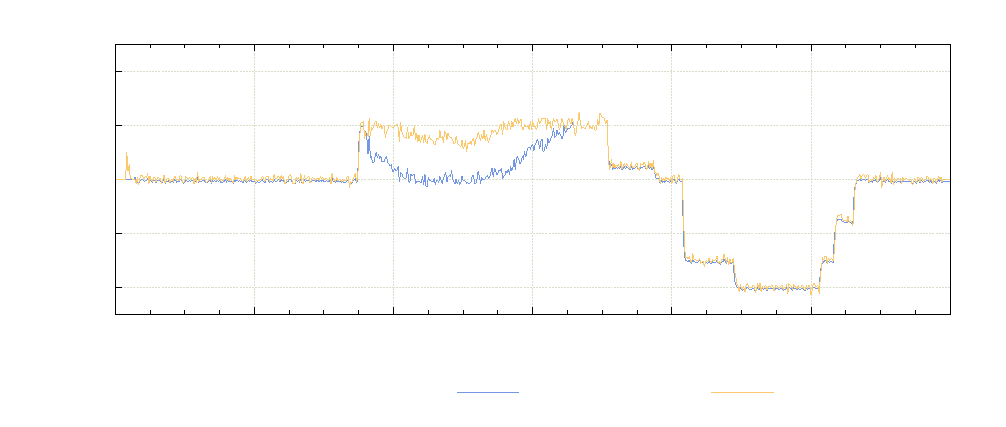
\includegraphics{Graphs/4/KUSResults/RefugePressure/RefugePressure}}%
    \gplfronttext
  \end{picture}%
\endgroup

		\caption{The Baseline system pressure compared to the system pressure when refuge bay leaks are reduce.}
		\label{fig: RefugeBay Pressures.}
	\end{figure}  
	Tested scenario where all excessive leaking valves are removed.
	Refuge bays savings 1MW E.E.
	
	\subsection{Scenario 2. Closing off levels vs. inactive work areas}
	Due to the high prevalence of compressed air misuse, leaks and open valves, significant amounts of air is still used during periods where it is not required. Reducing pressure to areas during the times may lead to a major power and cost saving. Using simulation, tests can be done to identify the benefits of reducing pressure to inactive mining sections.
	\par 
	The effect of in-stope control during peak times was simulated for level 105L. The level was modelled to include all major leaks, refuge bays and drilling sections that were manually identified from the level investigations. This is shown in the simulation diagram shown in Figure For comparison, station isolation and the combination of in-stope control and station isolation were simulated. 
	
	\begin{figure}[h!]
		\centering
		\fbox{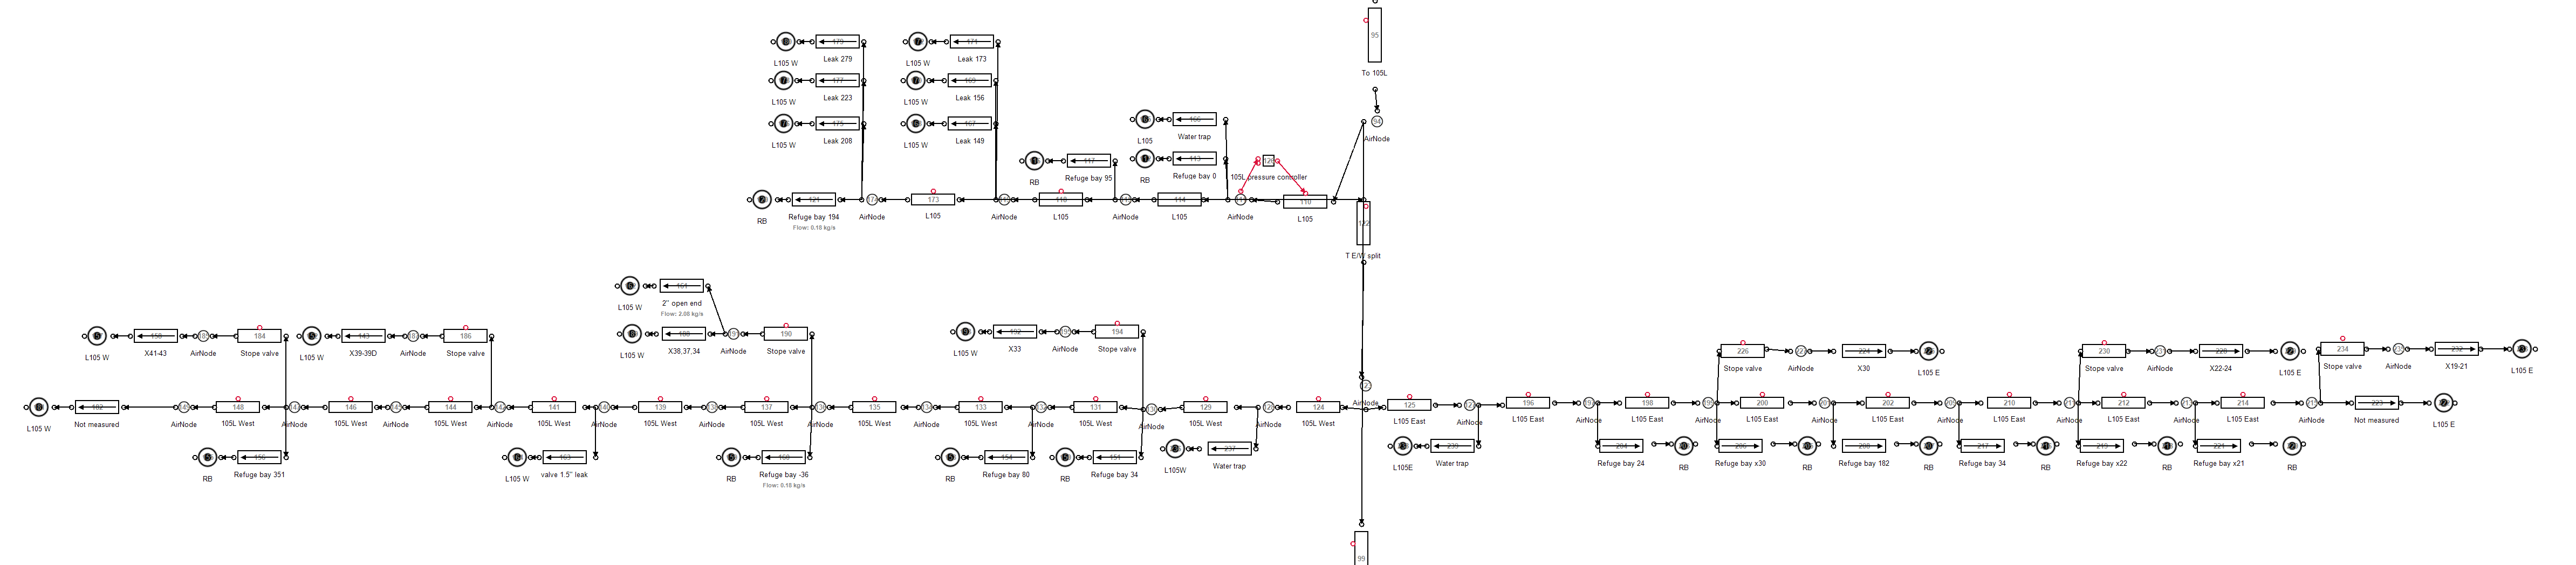
\includegraphics[width=\textwidth]{Images/4/StopeSim}}
		\caption{Underground level layout.}
		\label{fig: KUS Simulation level layout}
	\end{figure}	
	
	
	\subsection{Validation of results}
	
	- awaiting results on manual tests
	
	\subsection{Summary}
\newpage
\section{Case study C: Periodic simulation analysis}
	\subsection{Preamble}
	Updating the inputs of a simulation periodically could be used to verify simulation model accuracy. If the precision of simulation outputs remains for subsequent days, this would indicate that the model is correctly calibrated. Additionally, this process could be used to identify significant operational changes that occur within the system. This would cause the simulation outputs to differ from the actual measured parameters. 
	\par 
	A daily periodic simulation  analysis was implemented between 2016/11/01 and 2016/11/30 using the periodic simulation methodology discussed in Chapter 3. The simulation model developed for case study A was used for the analysis. The simulation receives the data inputs shown in table \ref{table: Periodic inputs/outputs}.
	\begin{table}[h]
		\centering
		\begin{tabular}{ll}
			\hline
			Inputs \hspace*{4cm}    &Outputs \hspace*{4cm}    \\  \hline
			Ambient air conditions&Compressor power \\
			Measured flows& Flows \\
			Compressor schedules& Pressures \\
			\hline
		\end{tabular}
		\caption{Data inputs and outputs for the simulation .}
		\label{table: Periodic inputs/outputs}
	\end{table}

\subsection{Results}


 The process was triggered daily. For each period, data inputs shown in table \ref{table: Periodic inputs/outputs} were imported into the model, the simulation was then processed and the outputs are compared with the real system parameters. Figure \ref{fig: Periodic simulation} shows the average daily accuracy of the simulated total system power, flow and the shaft pressure per period.
	     \par 
     
	\begin{figure}[h]
		\centering
		% GNUPLOT: LaTeX picture with Postscript
\begingroup
  \makeatletter
  \providecommand\color[2][]{%
    \GenericError{(gnuplot) \space\space\space\@spaces}{%
      Package color not loaded in conjunction with
      terminal option `colourtext'%
    }{See the gnuplot documentation for explanation.%
    }{Either use 'blacktext' in gnuplot or load the package
      color.sty in LaTeX.}%
    \renewcommand\color[2][]{}%
  }%
  \providecommand\includegraphics[2][]{%
    \GenericError{(gnuplot) \space\space\space\@spaces}{%
      Package graphicx or graphics not loaded%
    }{See the gnuplot documentation for explanation.%
    }{The gnuplot epslatex terminal needs graphicx.sty or graphics.sty.}%
    \renewcommand\includegraphics[2][]{}%
  }%
  \providecommand\rotatebox[2]{#2}%
  \@ifundefined{ifGPcolor}{%
    \newif\ifGPcolor
    \GPcolortrue
  }{}%
  \@ifundefined{ifGPblacktext}{%
    \newif\ifGPblacktext
    \GPblacktextfalse
  }{}%
  % define a \g@addto@macro without @ in the name:
  \let\gplgaddtomacro\g@addto@macro
  % define empty templates for all commands taking text:
  \gdef\gplbacktext{}%
  \gdef\gplfronttext{}%
  \makeatother
  \ifGPblacktext
    % no textcolor at all
    \def\colorrgb#1{}%
    \def\colorgray#1{}%
  \else
    % gray or color?
    \ifGPcolor
      \def\colorrgb#1{\color[rgb]{#1}}%
      \def\colorgray#1{\color[gray]{#1}}%
      \expandafter\def\csname LTw\endcsname{\color{white}}%
      \expandafter\def\csname LTb\endcsname{\color{black}}%
      \expandafter\def\csname LTa\endcsname{\color{black}}%
      \expandafter\def\csname LT0\endcsname{\color[rgb]{1,0,0}}%
      \expandafter\def\csname LT1\endcsname{\color[rgb]{0,1,0}}%
      \expandafter\def\csname LT2\endcsname{\color[rgb]{0,0,1}}%
      \expandafter\def\csname LT3\endcsname{\color[rgb]{1,0,1}}%
      \expandafter\def\csname LT4\endcsname{\color[rgb]{0,1,1}}%
      \expandafter\def\csname LT5\endcsname{\color[rgb]{1,1,0}}%
      \expandafter\def\csname LT6\endcsname{\color[rgb]{0,0,0}}%
      \expandafter\def\csname LT7\endcsname{\color[rgb]{1,0.3,0}}%
      \expandafter\def\csname LT8\endcsname{\color[rgb]{0.5,0.5,0.5}}%
    \else
      % gray
      \def\colorrgb#1{\color{black}}%
      \def\colorgray#1{\color[gray]{#1}}%
      \expandafter\def\csname LTw\endcsname{\color{white}}%
      \expandafter\def\csname LTb\endcsname{\color{black}}%
      \expandafter\def\csname LTa\endcsname{\color{black}}%
      \expandafter\def\csname LT0\endcsname{\color{black}}%
      \expandafter\def\csname LT1\endcsname{\color{black}}%
      \expandafter\def\csname LT2\endcsname{\color{black}}%
      \expandafter\def\csname LT3\endcsname{\color{black}}%
      \expandafter\def\csname LT4\endcsname{\color{black}}%
      \expandafter\def\csname LT5\endcsname{\color{black}}%
      \expandafter\def\csname LT6\endcsname{\color{black}}%
      \expandafter\def\csname LT7\endcsname{\color{black}}%
      \expandafter\def\csname LT8\endcsname{\color{black}}%
    \fi
  \fi
    \setlength{\unitlength}{0.0500bp}%
    \ifx\gptboxheight\undefined%
      \newlength{\gptboxheight}%
      \newlength{\gptboxwidth}%
      \newsavebox{\gptboxtext}%
    \fi%
    \setlength{\fboxrule}{0.5pt}%
    \setlength{\fboxsep}{1pt}%
\begin{picture}(9360.00,4032.00)%
    \gplgaddtomacro\gplbacktext{%
      \colorrgb{0.00,0.00,0.00}%
      \put(814,924){\makebox(0,0)[r]{\strut{}$80$}}%
      \colorrgb{0.00,0.00,0.00}%
      \put(814,1635){\makebox(0,0)[r]{\strut{}$85$}}%
      \colorrgb{0.00,0.00,0.00}%
      \put(814,2346){\makebox(0,0)[r]{\strut{}$90$}}%
      \colorrgb{0.00,0.00,0.00}%
      \put(814,3056){\makebox(0,0)[r]{\strut{}$95$}}%
      \colorrgb{0.00,0.00,0.00}%
      \put(814,3767){\makebox(0,0)[r]{\strut{}$100$}}%
      \colorrgb{0.00,0.00,0.00}%
      \put(946,704){\makebox(0,0){\strut{}2016/11/01}}%
      \colorrgb{0.00,0.00,0.00}%
      \put(2604,704){\makebox(0,0){\strut{}2016/11/07}}%
      \colorrgb{0.00,0.00,0.00}%
      \put(4263,704){\makebox(0,0){\strut{}2016/11/13}}%
      \colorrgb{0.00,0.00,0.00}%
      \put(5921,704){\makebox(0,0){\strut{}2016/11/19}}%
      \colorrgb{0.00,0.00,0.00}%
      \put(7580,704){\makebox(0,0){\strut{}2016/11/25}}%
    }%
    \gplgaddtomacro\gplfronttext{%
      \csname LTb\endcsname%
      \put(176,2345){\rotatebox{-270}{\makebox(0,0){\strut{}Accuracy (\%)}}}%
      \put(4954,374){\makebox(0,0){\strut{}Date of simulation}}%
      \csname LTb\endcsname%
      \put(3143,173){\makebox(0,0)[r]{\strut{}Flow}}%
      \csname LTb\endcsname%
      \put(5054,173){\makebox(0,0)[r]{\strut{}Pressure}}%
      \csname LTb\endcsname%
      \put(6965,173){\makebox(0,0)[r]{\strut{}Power}}%
    }%
    \gplbacktext
    \put(0,0){\fbox{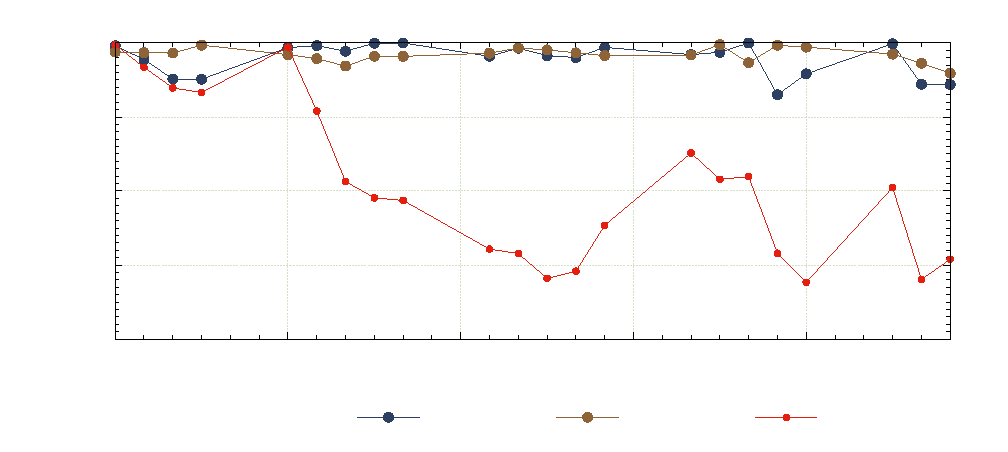
\includegraphics[trim=0 0 0.1cm 0, clip]{Graphs/4/Periodic1/Periodic1}}}%
    \gplfronttext
  \end{picture}%
\endgroup

		\caption{The flow, pressure and power error percentages for daily periodic simulations over a month.}
		\label{fig: Periodic simulation}
	\end{figure}   
The accuracy of the process parameters of the simulation was within 5\% for the duration of the periodic simulation. However, From the 2016/11/07, the accuracy of the simulated power dropped by between 10 and 15 percent. The daily average power of the system up to the point was approximately 12.5 MW, a 15\% simulation error therefore relates to 1.9 MW difference between simulated and actual parameters. This suggests a major shift in operation of the system.
\par 
An analysis was done to try determine the source of the discrepancy. From the data it was identified that the simulated power for compressor 1 was the source of the different A look at the actual power measurement for compressor 1 show drop compared to normal operation by almost 2 MW. At the same time the power used per kg/s of air seemed to have dropped. Figure \ref{fig: MeasurementAccuracy.} shows the average daily power for compressor 1 (blue), compared to the air mass flow per Watt(yellow). 
	\begin{figure}[h]
		\centering
		% GNUPLOT: LaTeX picture with Postscript
\begingroup
  \makeatletter
  \providecommand\color[2][]{%
    \GenericError{(gnuplot) \space\space\space\@spaces}{%
      Package color not loaded in conjunction with
      terminal option `colourtext'%
    }{See the gnuplot documentation for explanation.%
    }{Either use 'blacktext' in gnuplot or load the package
      color.sty in LaTeX.}%
    \renewcommand\color[2][]{}%
  }%
  \providecommand\includegraphics[2][]{%
    \GenericError{(gnuplot) \space\space\space\@spaces}{%
      Package graphicx or graphics not loaded%
    }{See the gnuplot documentation for explanation.%
    }{The gnuplot epslatex terminal needs graphicx.sty or graphics.sty.}%
    \renewcommand\includegraphics[2][]{}%
  }%
  \providecommand\rotatebox[2]{#2}%
  \@ifundefined{ifGPcolor}{%
    \newif\ifGPcolor
    \GPcolortrue
  }{}%
  \@ifundefined{ifGPblacktext}{%
    \newif\ifGPblacktext
    \GPblacktextfalse
  }{}%
  % define a \g@addto@macro without @ in the name:
  \let\gplgaddtomacro\g@addto@macro
  % define empty templates for all commands taking text:
  \gdef\gplbacktext{}%
  \gdef\gplfronttext{}%
  \makeatother
  \ifGPblacktext
    % no textcolor at all
    \def\colorrgb#1{}%
    \def\colorgray#1{}%
  \else
    % gray or color?
    \ifGPcolor
      \def\colorrgb#1{\color[rgb]{#1}}%
      \def\colorgray#1{\color[gray]{#1}}%
      \expandafter\def\csname LTw\endcsname{\color{white}}%
      \expandafter\def\csname LTb\endcsname{\color{black}}%
      \expandafter\def\csname LTa\endcsname{\color{black}}%
      \expandafter\def\csname LT0\endcsname{\color[rgb]{1,0,0}}%
      \expandafter\def\csname LT1\endcsname{\color[rgb]{0,1,0}}%
      \expandafter\def\csname LT2\endcsname{\color[rgb]{0,0,1}}%
      \expandafter\def\csname LT3\endcsname{\color[rgb]{1,0,1}}%
      \expandafter\def\csname LT4\endcsname{\color[rgb]{0,1,1}}%
      \expandafter\def\csname LT5\endcsname{\color[rgb]{1,1,0}}%
      \expandafter\def\csname LT6\endcsname{\color[rgb]{0,0,0}}%
      \expandafter\def\csname LT7\endcsname{\color[rgb]{1,0.3,0}}%
      \expandafter\def\csname LT8\endcsname{\color[rgb]{0.5,0.5,0.5}}%
    \else
      % gray
      \def\colorrgb#1{\color{black}}%
      \def\colorgray#1{\color[gray]{#1}}%
      \expandafter\def\csname LTw\endcsname{\color{white}}%
      \expandafter\def\csname LTb\endcsname{\color{black}}%
      \expandafter\def\csname LTa\endcsname{\color{black}}%
      \expandafter\def\csname LT0\endcsname{\color{black}}%
      \expandafter\def\csname LT1\endcsname{\color{black}}%
      \expandafter\def\csname LT2\endcsname{\color{black}}%
      \expandafter\def\csname LT3\endcsname{\color{black}}%
      \expandafter\def\csname LT4\endcsname{\color{black}}%
      \expandafter\def\csname LT5\endcsname{\color{black}}%
      \expandafter\def\csname LT6\endcsname{\color{black}}%
      \expandafter\def\csname LT7\endcsname{\color{black}}%
      \expandafter\def\csname LT8\endcsname{\color{black}}%
    \fi
  \fi
    \setlength{\unitlength}{0.0500bp}%
    \ifx\gptboxheight\undefined%
      \newlength{\gptboxheight}%
      \newlength{\gptboxwidth}%
      \newsavebox{\gptboxtext}%
    \fi%
    \setlength{\fboxrule}{0.5pt}%
    \setlength{\fboxsep}{1pt}%
\begin{picture}(9360.00,3528.00)%
    \gplgaddtomacro\gplbacktext{%
      \colorrgb{0.00,0.00,0.00}%
      \put(946,924){\makebox(0,0)[r]{\strut{}$1000$}}%
      \colorrgb{0.00,0.00,0.00}%
      \put(946,1314){\makebox(0,0)[r]{\strut{}$1500$}}%
      \colorrgb{0.00,0.00,0.00}%
      \put(946,1704){\makebox(0,0)[r]{\strut{}$2000$}}%
      \colorrgb{0.00,0.00,0.00}%
      \put(946,2094){\makebox(0,0)[r]{\strut{}$2500$}}%
      \colorrgb{0.00,0.00,0.00}%
      \put(946,2483){\makebox(0,0)[r]{\strut{}$3000$}}%
      \colorrgb{0.00,0.00,0.00}%
      \put(946,2873){\makebox(0,0)[r]{\strut{}$3500$}}%
      \colorrgb{0.00,0.00,0.00}%
      \put(946,3263){\makebox(0,0)[r]{\strut{}$4000$}}%
      \colorrgb{0.00,0.00,0.00}%
      \put(1078,704){\makebox(0,0){\strut{}2016/09/01}}%
      \colorrgb{0.00,0.00,0.00}%
      \put(3118,704){\makebox(0,0){\strut{}2016/10/01}}%
      \colorrgb{0.00,0.00,0.00}%
      \put(5226,704){\makebox(0,0){\strut{}2016/11/01}}%
      \colorrgb{0.00,0.00,0.00}%
      \put(5226,704){\makebox(0,0){\strut{}2016/11/01}}%
      \colorrgb{0.00,0.00,0.00}%
      \put(7266,704){\makebox(0,0){\strut{}2016/12/01}}%
      \colorrgb{0.00,0.00,0.00}%
      \put(8214,924){\makebox(0,0)[l]{\strut{}$2$}}%
      \colorrgb{0.00,0.00,0.00}%
      \put(8214,1314){\makebox(0,0)[l]{\strut{}$2.5$}}%
      \colorrgb{0.00,0.00,0.00}%
      \put(8214,1704){\makebox(0,0)[l]{\strut{}$3$}}%
      \colorrgb{0.00,0.00,0.00}%
      \put(8214,2094){\makebox(0,0)[l]{\strut{}$3.5$}}%
      \colorrgb{0.00,0.00,0.00}%
      \put(8214,2483){\makebox(0,0)[l]{\strut{}$4$}}%
      \colorrgb{0.00,0.00,0.00}%
      \put(8214,2873){\makebox(0,0)[l]{\strut{}$4.5$}}%
      \colorrgb{0.00,0.00,0.00}%
      \put(8214,3263){\makebox(0,0)[l]{\strut{}$5$}}%
    }%
    \gplgaddtomacro\gplfronttext{%
      \csname LTb\endcsname%
      \put(176,2093){\rotatebox{-270}{\makebox(0,0){\strut{}Power (kW)}}}%
      \put(8851,2093){\rotatebox{-270}{\makebox(0,0){\strut{}$Flow per Watt (kg/s/W)$}}}%
      \put(4580,374){\makebox(0,0){\strut{}Date}}%
      \csname LTb\endcsname%
      \put(3725,173){\makebox(0,0)[r]{\strut{}Compressor 1 average power}}%
      \csname LTb\endcsname%
      \put(8012,173){\makebox(0,0)[r]{\strut{}System efficiency}}%
      \csname LTb\endcsname%
      \put(6220,3029){\makebox(0,0){\strut{}\shortstack{\small{Periodic simulation}}}}%
    }%
    \gplbacktext
    \put(0,0){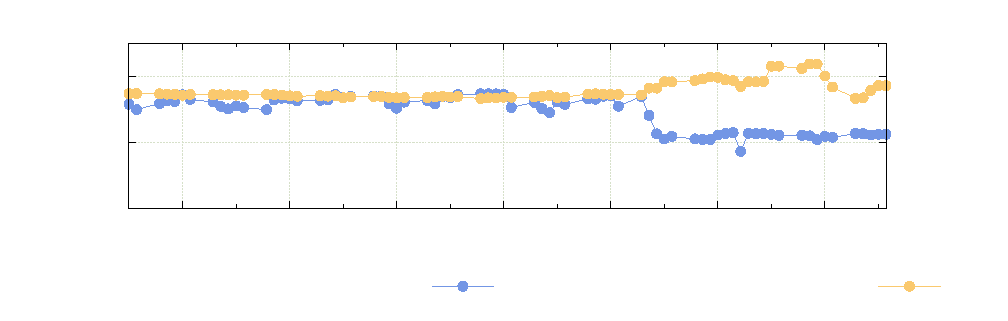
\includegraphics{Graphs/4/PeriodicRange/PeriodicRange}}%
    \gplfronttext
  \end{picture}%
\endgroup

		\caption{Supply efficiency and Compressor 1's average power output over the time of the periodic analysis.}
		\label{fig: MeasurementAccuracy.}
	\end{figure} 
As a 2 MW shift in power is not likely from, the results seem to show that there was a fault in the power metering starting from 2016/11/07. This explains the perceived increase in efficiency over the same period as a less power is measure then is actually being provided. In this situation the simulated power measurement is actually a more accurate metric for compressor 1's power over this period.  
   \subsection{Validation}
To validate that the change identified using periodic simulation was caused by the power meter, data from the substation was compared to the combined individual compressors meters. This comparison is shown in Figure \ref{fig: Corrected Periodic simulation}. The comparison shows that the substation power measurement strays from the compressors at the same time that compressor 1 average daily power drops.
	\begin{figure}[h]
		\centering
		% GNUPLOT: LaTeX picture with Postscript
\begingroup
  \makeatletter
  \providecommand\color[2][]{%
    \GenericError{(gnuplot) \space\space\space\@spaces}{%
      Package color not loaded in conjunction with
      terminal option `colourtext'%
    }{See the gnuplot documentation for explanation.%
    }{Either use 'blacktext' in gnuplot or load the package
      color.sty in LaTeX.}%
    \renewcommand\color[2][]{}%
  }%
  \providecommand\includegraphics[2][]{%
    \GenericError{(gnuplot) \space\space\space\@spaces}{%
      Package graphicx or graphics not loaded%
    }{See the gnuplot documentation for explanation.%
    }{The gnuplot epslatex terminal needs graphicx.sty or graphics.sty.}%
    \renewcommand\includegraphics[2][]{}%
  }%
  \providecommand\rotatebox[2]{#2}%
  \@ifundefined{ifGPcolor}{%
    \newif\ifGPcolor
    \GPcolortrue
  }{}%
  \@ifundefined{ifGPblacktext}{%
    \newif\ifGPblacktext
    \GPblacktextfalse
  }{}%
  % define a \g@addto@macro without @ in the name:
  \let\gplgaddtomacro\g@addto@macro
  % define empty templates for all commands taking text:
  \gdef\gplbacktext{}%
  \gdef\gplfronttext{}%
  \makeatother
  \ifGPblacktext
    % no textcolor at all
    \def\colorrgb#1{}%
    \def\colorgray#1{}%
  \else
    % gray or color?
    \ifGPcolor
      \def\colorrgb#1{\color[rgb]{#1}}%
      \def\colorgray#1{\color[gray]{#1}}%
      \expandafter\def\csname LTw\endcsname{\color{white}}%
      \expandafter\def\csname LTb\endcsname{\color{black}}%
      \expandafter\def\csname LTa\endcsname{\color{black}}%
      \expandafter\def\csname LT0\endcsname{\color[rgb]{1,0,0}}%
      \expandafter\def\csname LT1\endcsname{\color[rgb]{0,1,0}}%
      \expandafter\def\csname LT2\endcsname{\color[rgb]{0,0,1}}%
      \expandafter\def\csname LT3\endcsname{\color[rgb]{1,0,1}}%
      \expandafter\def\csname LT4\endcsname{\color[rgb]{0,1,1}}%
      \expandafter\def\csname LT5\endcsname{\color[rgb]{1,1,0}}%
      \expandafter\def\csname LT6\endcsname{\color[rgb]{0,0,0}}%
      \expandafter\def\csname LT7\endcsname{\color[rgb]{1,0.3,0}}%
      \expandafter\def\csname LT8\endcsname{\color[rgb]{0.5,0.5,0.5}}%
    \else
      % gray
      \def\colorrgb#1{\color{black}}%
      \def\colorgray#1{\color[gray]{#1}}%
      \expandafter\def\csname LTw\endcsname{\color{white}}%
      \expandafter\def\csname LTb\endcsname{\color{black}}%
      \expandafter\def\csname LTa\endcsname{\color{black}}%
      \expandafter\def\csname LT0\endcsname{\color{black}}%
      \expandafter\def\csname LT1\endcsname{\color{black}}%
      \expandafter\def\csname LT2\endcsname{\color{black}}%
      \expandafter\def\csname LT3\endcsname{\color{black}}%
      \expandafter\def\csname LT4\endcsname{\color{black}}%
      \expandafter\def\csname LT5\endcsname{\color{black}}%
      \expandafter\def\csname LT6\endcsname{\color{black}}%
      \expandafter\def\csname LT7\endcsname{\color{black}}%
      \expandafter\def\csname LT8\endcsname{\color{black}}%
    \fi
  \fi
    \setlength{\unitlength}{0.0500bp}%
    \ifx\gptboxheight\undefined%
      \newlength{\gptboxheight}%
      \newlength{\gptboxwidth}%
      \newsavebox{\gptboxtext}%
    \fi%
    \setlength{\fboxrule}{0.5pt}%
    \setlength{\fboxsep}{1pt}%
\begin{picture}(9360.00,4284.00)%
    \gplgaddtomacro\gplbacktext{%
      \colorrgb{0.00,0.00,0.00}%
      \put(682,1366){\makebox(0,0)[r]{\strut{}$8$}}%
      \colorrgb{0.00,0.00,0.00}%
      \put(682,2250){\makebox(0,0)[r]{\strut{}$10$}}%
      \colorrgb{0.00,0.00,0.00}%
      \put(682,3135){\makebox(0,0)[r]{\strut{}$12$}}%
      \colorrgb{0.00,0.00,0.00}%
      \put(682,4019){\makebox(0,0)[r]{\strut{}$14$}}%
      \colorrgb{0.00,0.00,0.00}%
      \put(1938,704){\makebox(0,0){\strut{}05/11/2016}}%
      \colorrgb{0.00,0.00,0.00}%
      \put(3343,704){\makebox(0,0){\strut{}10/11/2016}}%
      \colorrgb{0.00,0.00,0.00}%
      \put(4748,704){\makebox(0,0){\strut{}15/11/2016}}%
      \colorrgb{0.00,0.00,0.00}%
      \put(6152,704){\makebox(0,0){\strut{}20/11/2016}}%
      \colorrgb{0.00,0.00,0.00}%
      \put(7557,704){\makebox(0,0){\strut{}25/11/2016}}%
      \colorrgb{0.00,0.00,0.00}%
      \put(8962,704){\makebox(0,0){\strut{}30/11/2016}}%
    }%
    \gplgaddtomacro\gplfronttext{%
      \csname LTb\endcsname%
      \put(176,2471){\rotatebox{-270}{\makebox(0,0){\strut{}Power (MW)}}}%
      \put(4888,374){\makebox(0,0){\strut{}Date}}%
      \csname LTb\endcsname%
      \put(4033,173){\makebox(0,0)[r]{\strut{}Compressor power measrement}}%
      \csname LTb\endcsname%
      \put(8452,173){\makebox(0,0)[r]{\strut{}Independant measurement}}%
    }%
    \gplbacktext
    \put(0,0){\fbox{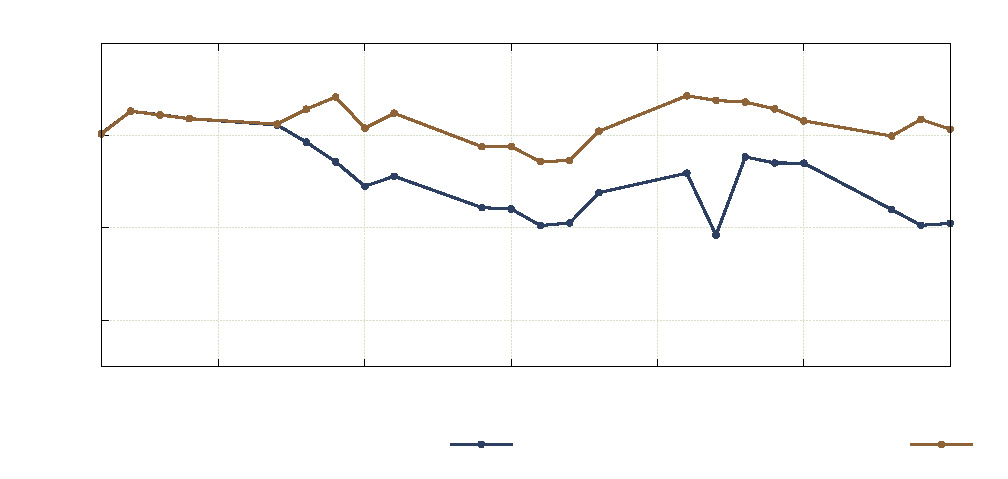
\includegraphics[trim=0 0 0.1cm 0, clip]{Graphs/4/PeriodicValidation/PeriodicValidation}}}%
    \gplfronttext
  \end{picture}%
\endgroup

		\caption{Comparison using alternative power source.}
		\label{fig: Corrected Periodic simulation}
	\end{figure}    
	
	\subsection{Summary}
\newpage
\section{Potential benefit for SA mines}

	Using  
\section{Conclusion}